\chapter[Revisión literaria]{Revisión literaria\label{cap:revision}}

\section{Marco teórico}

\label{sec:physics}

\subsection{Heliofísica, regiones activas y clima espacial}

La heliofísica estudia los procesos físicos que gobiernan la interacción entre el Sol, la heliosfera y el entorno espacial terrestre. Esta disciplina integra fenómenos magnetohidrodinámicos, electromagnéticos y de transporte de energía que vinculan la actividad solar con las condiciones del medio interplanetario y sus efectos sobre la Tierra.

El Sol es una estrella magnéticamente activa cuya dinámica interna genera campos magnéticos que emergen continuamente hacia su superficie visible, denominada fotosfera. La concentración y reorganización de estos campos da lugar a estructuras conocidas como regiones activas, caracterizadas por una intensa actividad magnética y frecuentemente asociadas a grupos de manchas solares. Estas regiones constituyen los principales reservorios de energía magnética libre de la atmósfera solar y representan los sitios donde se originan los fenómenos eruptivos más energéticos del Sol, principalmente las fulguraciones solares (\textit{solar flares}) y las Eyecciones de Masa Coronal (CME, por sus siglas en inglés), ambos considerados impulsores fundamentales del clima espacial \citep{hathaway2010solarcycle,usaf2003sunspot}.


\begin{figure}[H]
\centering
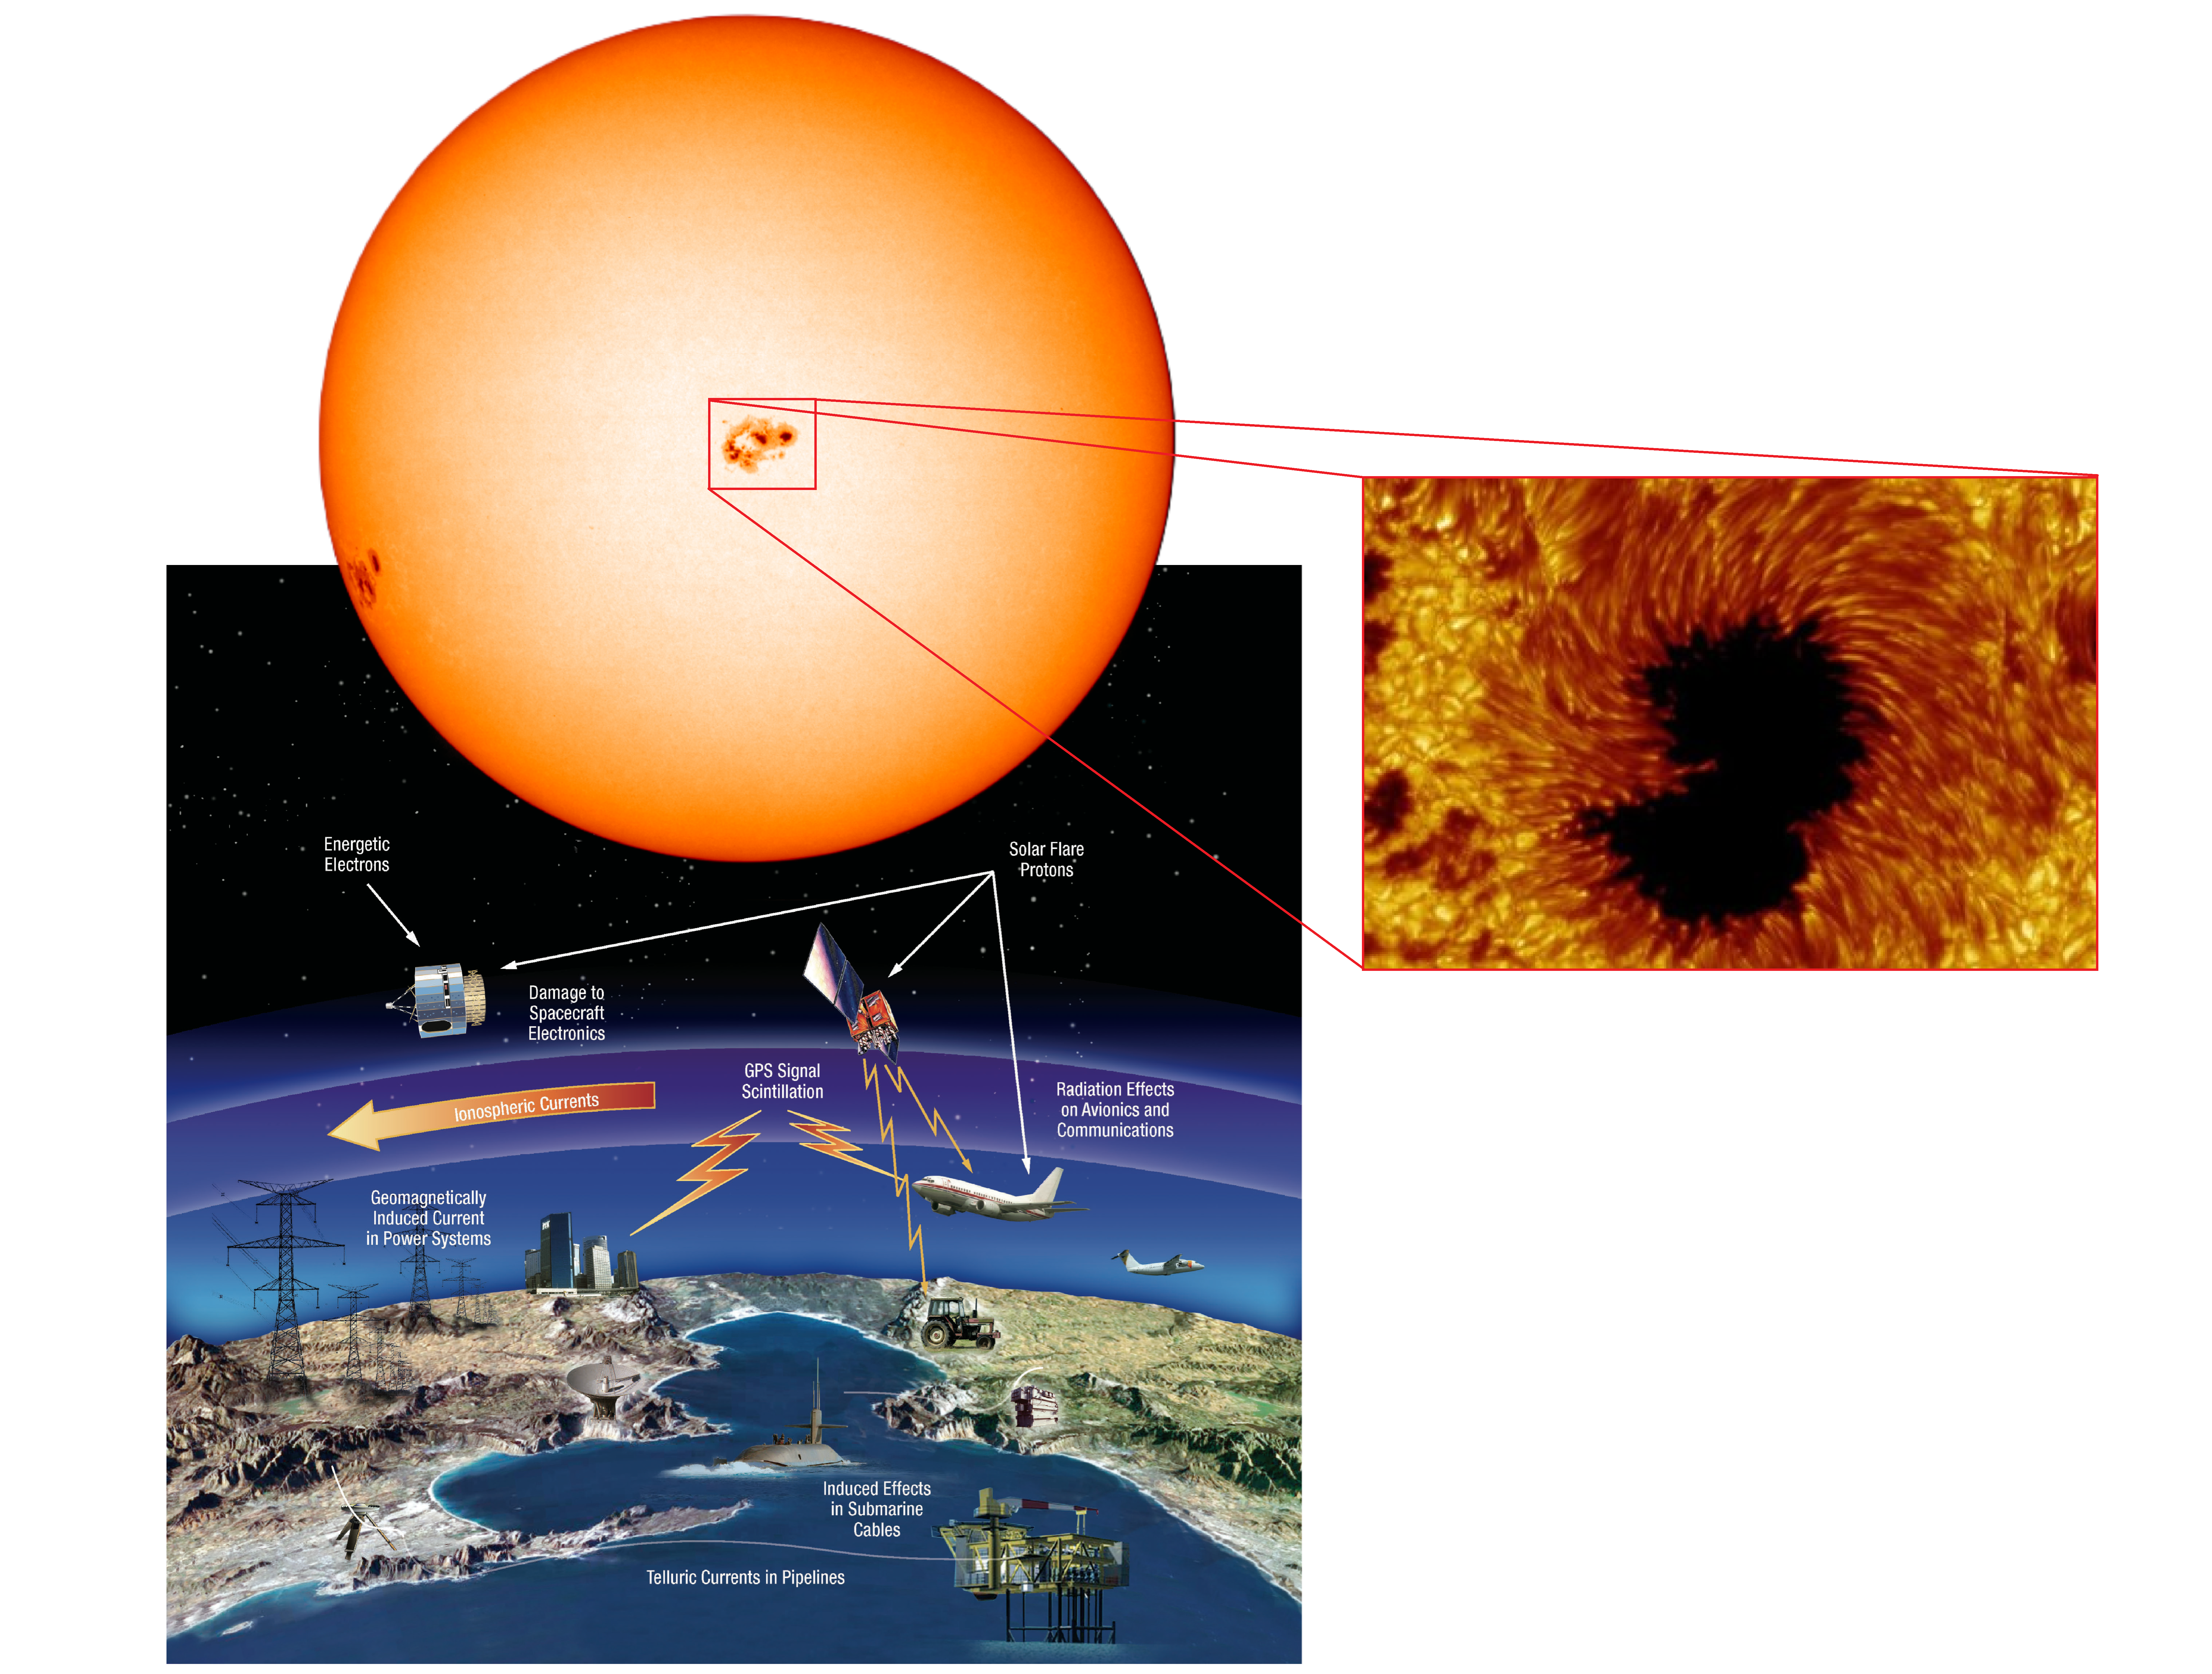
\includegraphics[width=0.85\textwidth]{figures/solar/space-weather-effects.png}
\caption{Diagrama de los principales efectos del clima espacial sobre sistemas tecnológicos y el entorno terrestre (NASA SVS). \textbf{Fuente:} NASA Scientific Visualization Studio.}
\label{fig:}
\end{figure}

La influencia de estos eventos sobre la Tierra sigue una secuencia física bien establecida. Las fulguraciones solares emiten radiación electromagnética a lo largo de un amplio espectro de frecuencias que alcanza la Tierra aproximadamente ocho minutos después de su emisión, produciendo alteraciones en la ionosfera. Por su parte, las CME expulsan grandes cantidades de plasma magnetizado al medio interplanetario. Cuando estas estructuras interactúan con la magnetosfera terrestre, pueden transferir energía, masa y momento al sistema magnetosférico mediante procesos de reconexión magnética, particularmente cuando la orientación del campo magnético interplanetario favorece el acoplamiento con el campo geomagnético terrestre \citep{spaceaustralia2026}. Como resultado, se desencadenan procesos de aceleración y transporte de partículas energéticas a lo largo de las líneas de campo magnético \citep{reyes2021geomagnetic}.

La energía inyectada durante estos procesos puede dar lugar a tormentas geomagnéticas cuyos efectos se manifiestan sobre diversos sistemas tecnológicos críticos:

\begin{itemize}
\item \textbf{Expansión atmosférica y aumento del arrastre satelital:} La deposición de energía en la termosfera incrementa su temperatura y provoca una expansión de las capas atmosféricas superiores. Como consecuencia, aumenta la densidad atmosférica a altitudes orbitales bajas, incrementando el arrastre atmosférico sobre satélites artificiales y modificando sus parámetros orbitales \citep{spaceaustralia2026}.

\item \textbf{Degradación de sistemas de telecomunicación y posicionamiento:} Las perturbaciones ionosféricas alteran la propagación de ondas de radio, ocasionando interrupciones en enlaces de alta frecuencia e introduciendo errores de retardo y fase en señales de navegación satelital, afectando la precisión de sistemas GPS y GNSS \citep{spaceaustralia2026,grodji2021study}.

\item \textbf{Corrientes inducidas geomagnéticamente (GIC):} Las variaciones temporales del campo geomagnético inducen campos eléctricos sobre la superficie terrestre, generando corrientes en infraestructuras conductoras extensas, como redes eléctricas de transmisión. Estas corrientes pueden provocar saturación parcial de transformadores y comprometer la estabilidad operativa de los sistemas de potencia \citep{spaceaustralia2026}.

\end{itemize}

Bajo este escenario, el monitoreo continuo de las manchas solares trasciende el interés puramente observacional. El número de manchas solares (\textit{Sunspot Number}, SSN) constituye uno de los indicadores indirectos más utilizados de la actividad magnética global del Sol, mientras que la morfología y evolución de las regiones activas proporcionan información relevante sobre el potencial eruptivo de la atmósfera solar.

\begin{figure}[H]
\centering
\begin{subfigure}[t]{0.31\textwidth}
\centering
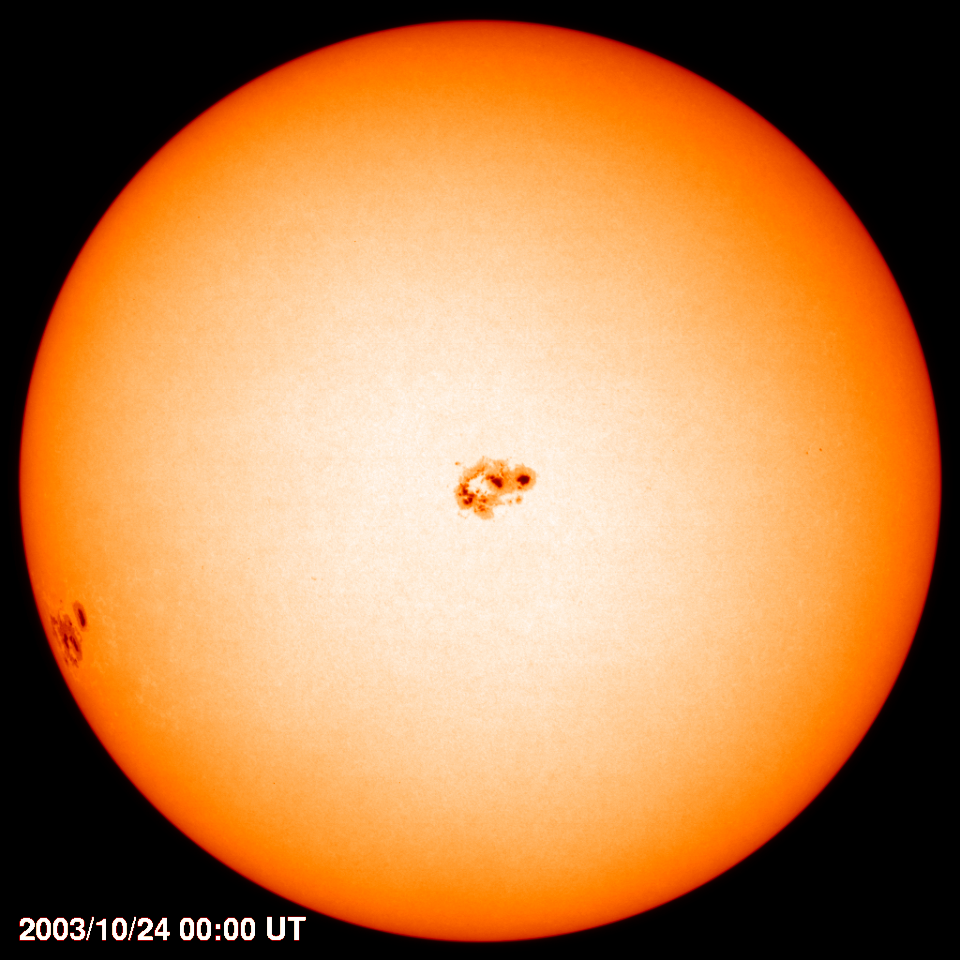
\includegraphics[width=\textwidth]{figures/solar/sunspot.png}
\caption{Imagen del disco solar completo.}
\end{subfigure}
\hfill
\begin{subfigure}[t]{0.44\textwidth}
\centering
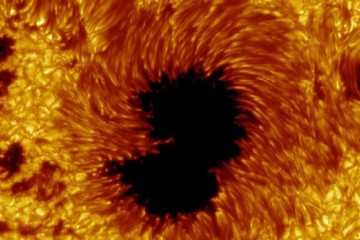
\includegraphics[width=\textwidth]{figures/solar/spot_close.jpg}
\caption{Detalles ampliados de una mancha solar.}
\end{subfigure}
\caption{Caracterización multiescala de la actividad solar: (a) disco solar completo con grupos activos fotosféricos; (b) detalle estructural de una mancha solar individual. \textbf{Fuente:} Solar Dynamics Observatory (SDO/NASA).}
\label{fig:teoria-sunspot}
\end{figure}

El estudio automatizado de estas estructuras fotosféricas permite relacionar características observacionales de las regiones activas con la probabilidad de ocurrencia de fenómenos eruptivos, incluyendo fulguraciones y eyecciones de masa coronal potencialmente geoefectivas. Esta capacidad resulta fundamental para el desarrollo de sistemas de monitoreo y modelos predictivos orientados a la caracterización del clima espacial.

\subsection{Herramientas observacionales y modalidades de observación}

La fotosfera es la capa visible del Sol y corresponde a la región desde la cual se emite la mayor parte de la radiación observada en continuo visible. En ella se reconocen estructuras como la granulación, la umbra y la penumbra de las manchas solares, por lo que constituye la referencia principal para la observación en luz blanca.

\begin{figure}[H]
  \centering
  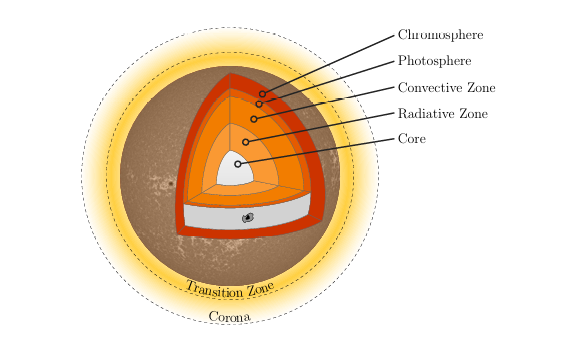
\includegraphics[width=0.76\textwidth]{figures/solar/sun_parts.png}
  \caption{Esquema general de las principales capas y regiones del Sol. La figura permite ubicar la fotosfera, cromosfera y corona dentro del contexto físico de las modalidades observacionales empleadas en heliofísica. \textbf{Fuente:} Adaptado de Sayez et al..}
  \label{fig:partes-sol}
\end{figure}

Por encima de la fotosfera se encuentra la cromosfera, una capa más tenue y estructurada por la interacción entre plasma y campo magnético, donde se observan plages, filamentos y otras manifestaciones asociadas a regiones activas. En consecuencia, la fotosfera se estudia habitualmente mediante luz blanca o continuo visible, mientras que la cromosfera suele analizarse a través de líneas espectrales como CaII K y H$\alpha$. 

Estas modalidades no son equivalentes ni redundantes. La luz blanca enfatiza umbra, penumbra y estructura fotosférica; CaII K revela plages asociadas a concentraciones de campo magnético; y H$\alpha$ muestra estructuras cromosféricas ligadas a la interacción plasma--campo.

\begin{figure}[H]
  \centering
  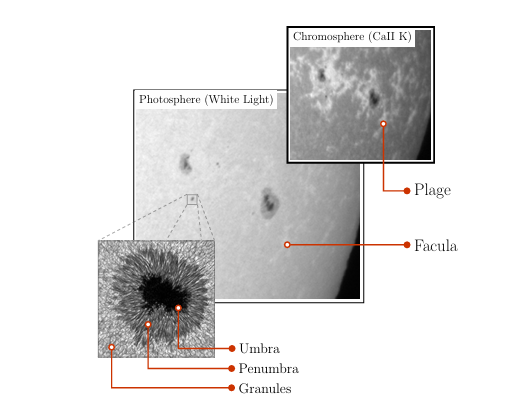
\includegraphics[width=0.82\textwidth]{figures/solar/wl_cak.png}
  \caption{Comparación observacional entre imágenes solares en luz blanca y CaII K. La figura ilustra cómo cada modalidad resalta estructuras distintas de la actividad solar. \textbf{Fuente:} Adaptado de Sayez et al..}
  \label{fig:wl-vs-caiik}
\end{figure}

Esta distinción resulta importante porque sitúa la clasificación de manchas solares dentro de un marco observacional más amplio. Aunque la presente tesis se enfoca principalmente en imágenes heliográficas de luz blanca, la interpretación física y observacional de dichas imágenes se beneficia del hecho de que forman parte de un ecosistema multibanda donde diferentes instrumentos revelan distintas capas y manifestaciones de la actividad solar \citep{scherrer2012hmi,bobra2014sharp}.

\subsection{Observatorios terrestres y elementos atmosféricos}

Las observaciones terrestres muestran que el monitoreo solar comenzó con proyecciones telescópicas y dibujos, y que evolucionó hacia observatorios equipados con telescopios ópticos, sensores digitales y, en algunos casos, arreglos distribuidos para observación sinótica. Dentro de esta categoría se mencionan, entre otros, redes globales como GONG y estaciones solares de larga duración como el Uccle Solar Equatorial Table (USET) del Observatorio Real de Bélgica. Estos sistemas son relevantes porque combinan seguimiento instrumental del Sol, continuidad temporal de registros y disponibilidad de productos útiles para contrastar procedimientos de análisis automático \citep{nsoGONG2026,robUSET2026,sidcGroundObservations2026}.

En el caso de USET, la referencia es principalmente metodológica e histórica. La estación opera una mesa ecuatorial con telescopios dedicados a observaciones en luz blanca, H$\alpha$ y CaII K, además de una tradición prolongada de dibujos solares y catálogos derivados. Por ello, USET permite ilustrar cómo un observatorio terrestre puede integrar adquisición digital, observación visual, anotación humana y preservación de metadatos dentro de una misma cadena observacional \citep{robUSET2026,sidcGroundObservations2026}.

\begin{figure}[H]
  \centering
  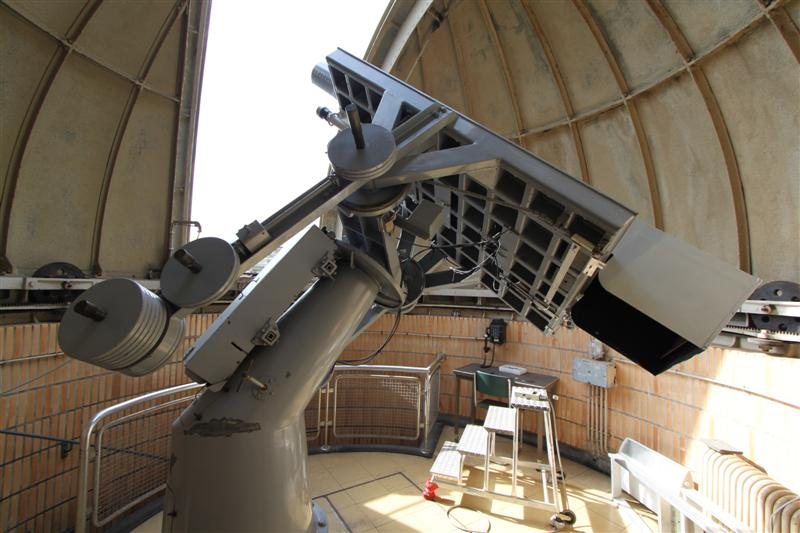
\includegraphics[width=0.78\textwidth]{figures/solar/scope_proj.jpg}
  \caption{Instalación instrumental del Uccle Solar Equatorial Table (USET), empleada para el seguimiento terrestre sistemático del Sol en distintas modalidades observacionales. \textbf{Fuente:} página oficial del Observatorio Real de Bélgica.}
  \label{fig:uset-instrument}
\end{figure}

A diferencia de esa referencia internacional, el contexto operativo directo de esta tesis se atribuye al Observatorio Astronómico ``Prof. Alexis Troche Boggino'', espacio académico de observación, formación y apoyo a actividades astronómicas asociado a la Facultad Politécnica de la Universidad Nacional de Asunción. Este entorno proporciona la referencia institucional y práctica para el desarrollo del prototipo, ya que permite vincular la adquisición de imágenes solares con una infraestructura real de observación, supervisión y registro.

La Figura~\ref{fig:observatorio-alexis-troche} muestra dicho contexto local. La subfigura (a) corresponde a la sala de control del Observatorio Astronómico ``Prof. Alexis Troche Boggino'', desde donde se supervisan actividades instrumentales y de observación; la subfigura (b) presenta el telescopio principal del observatorio. Aunque esta infraestructura principal define el entorno institucional y observacional del trabajo, para el desarrollo del prototipo se considera el uso de un telescopio refractor Vixen con diámetro $D=60\,\mathrm{mm}$ y distancia focal $F=420\,\mathrm{mm}$ como plataforma óptica de prueba, lo que permite trabajar con una configuración más compacta, segura y controlable durante las etapas de integración de cámara, filtrado solar, preprocesamiento local y validación inicial.

\begin{figure}[H]
    \centering
    \begin{subfigure}[t]{0.65\textwidth}
        \centering
        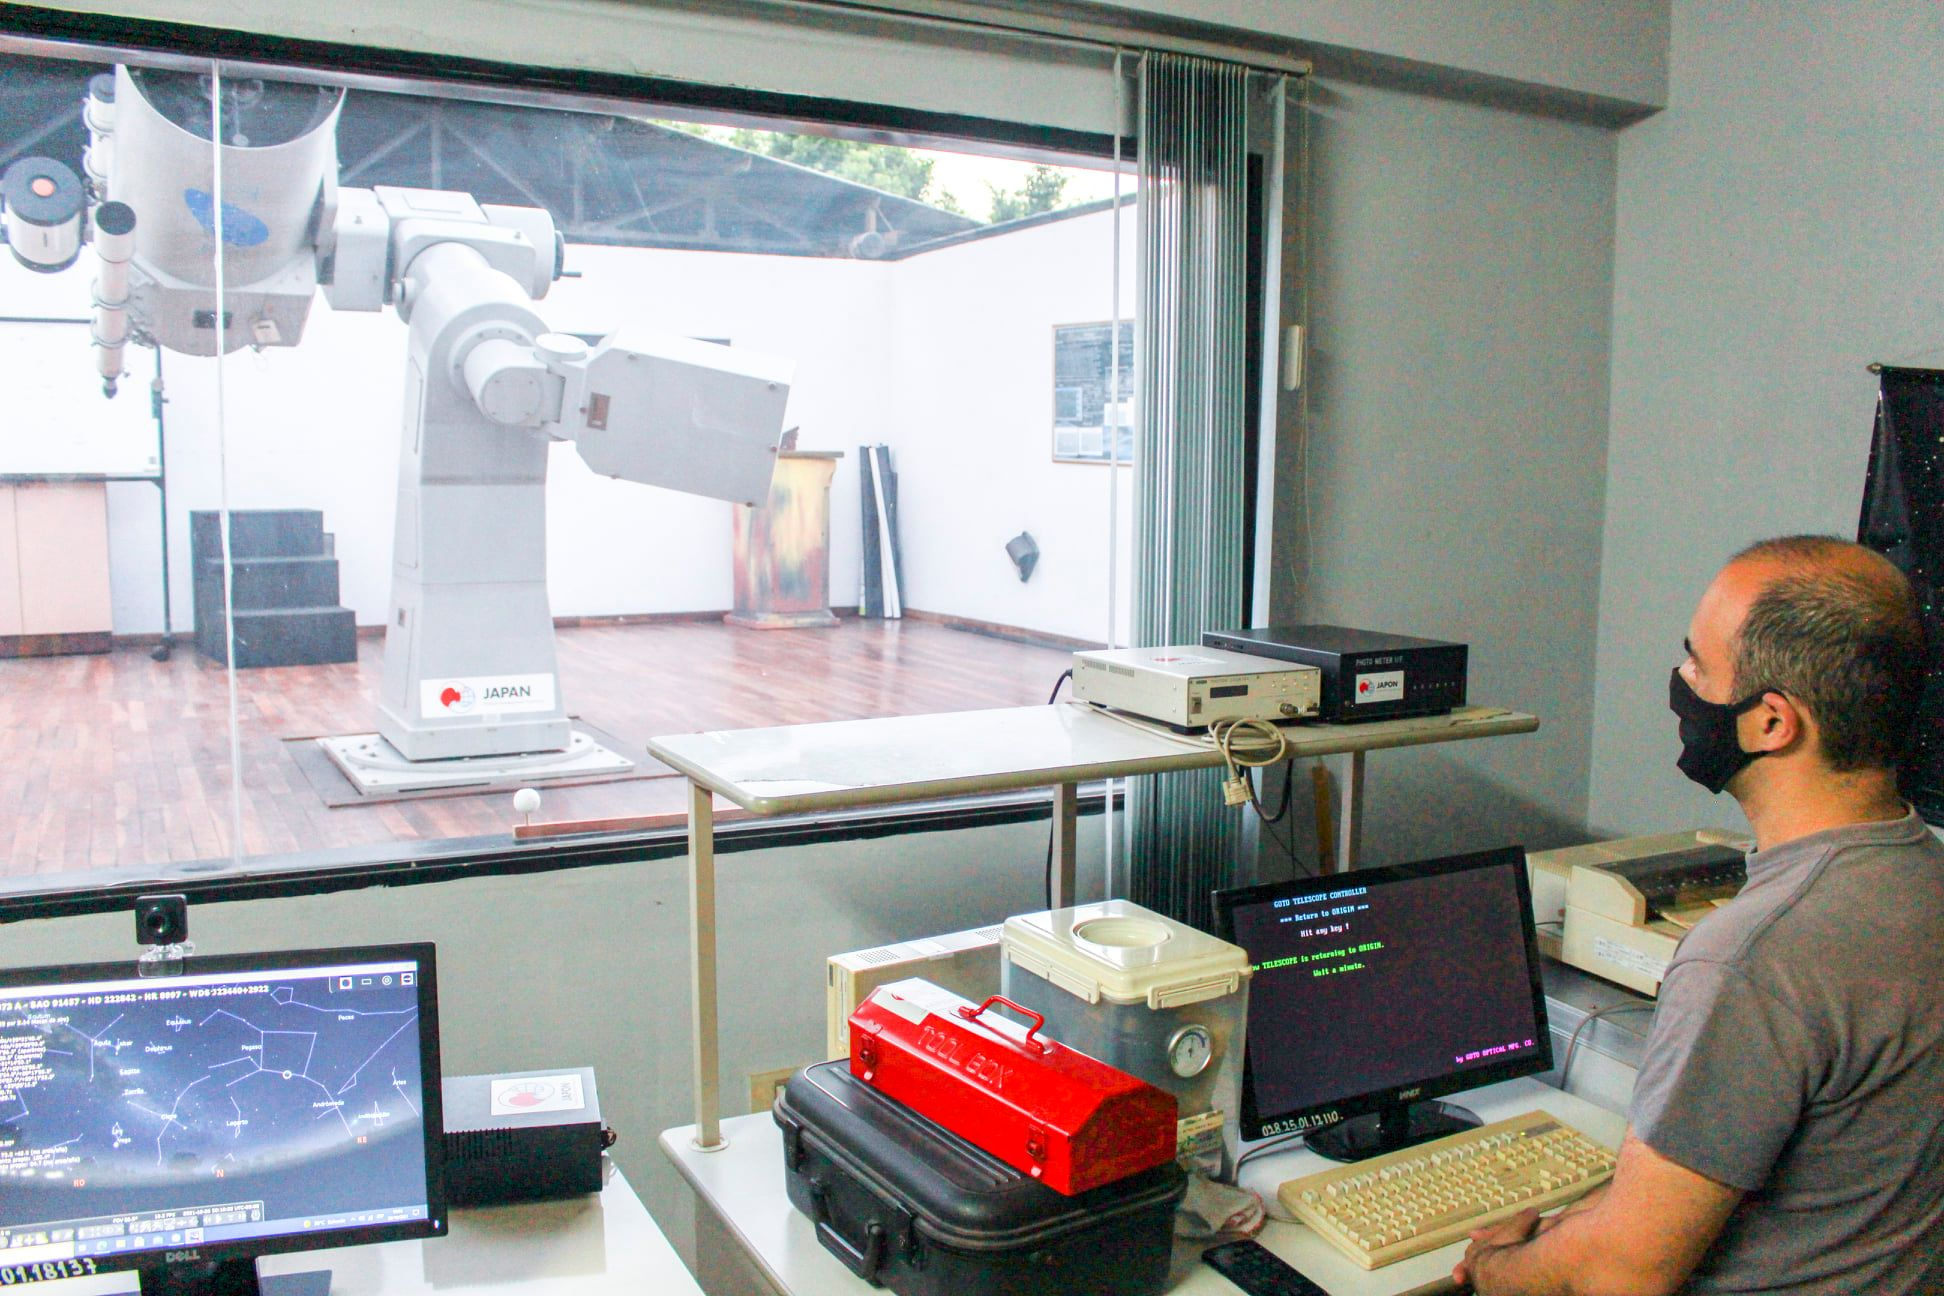
\includegraphics[width=\textwidth]{figures/obs/control.jpg}
        \caption{Sala de control del Observatorio Astronómico ``Prof. Alexis Troche Boggino''.}
    \end{subfigure}
    \hfill
    \begin{subfigure}[t]{0.30\textwidth}
        \centering
        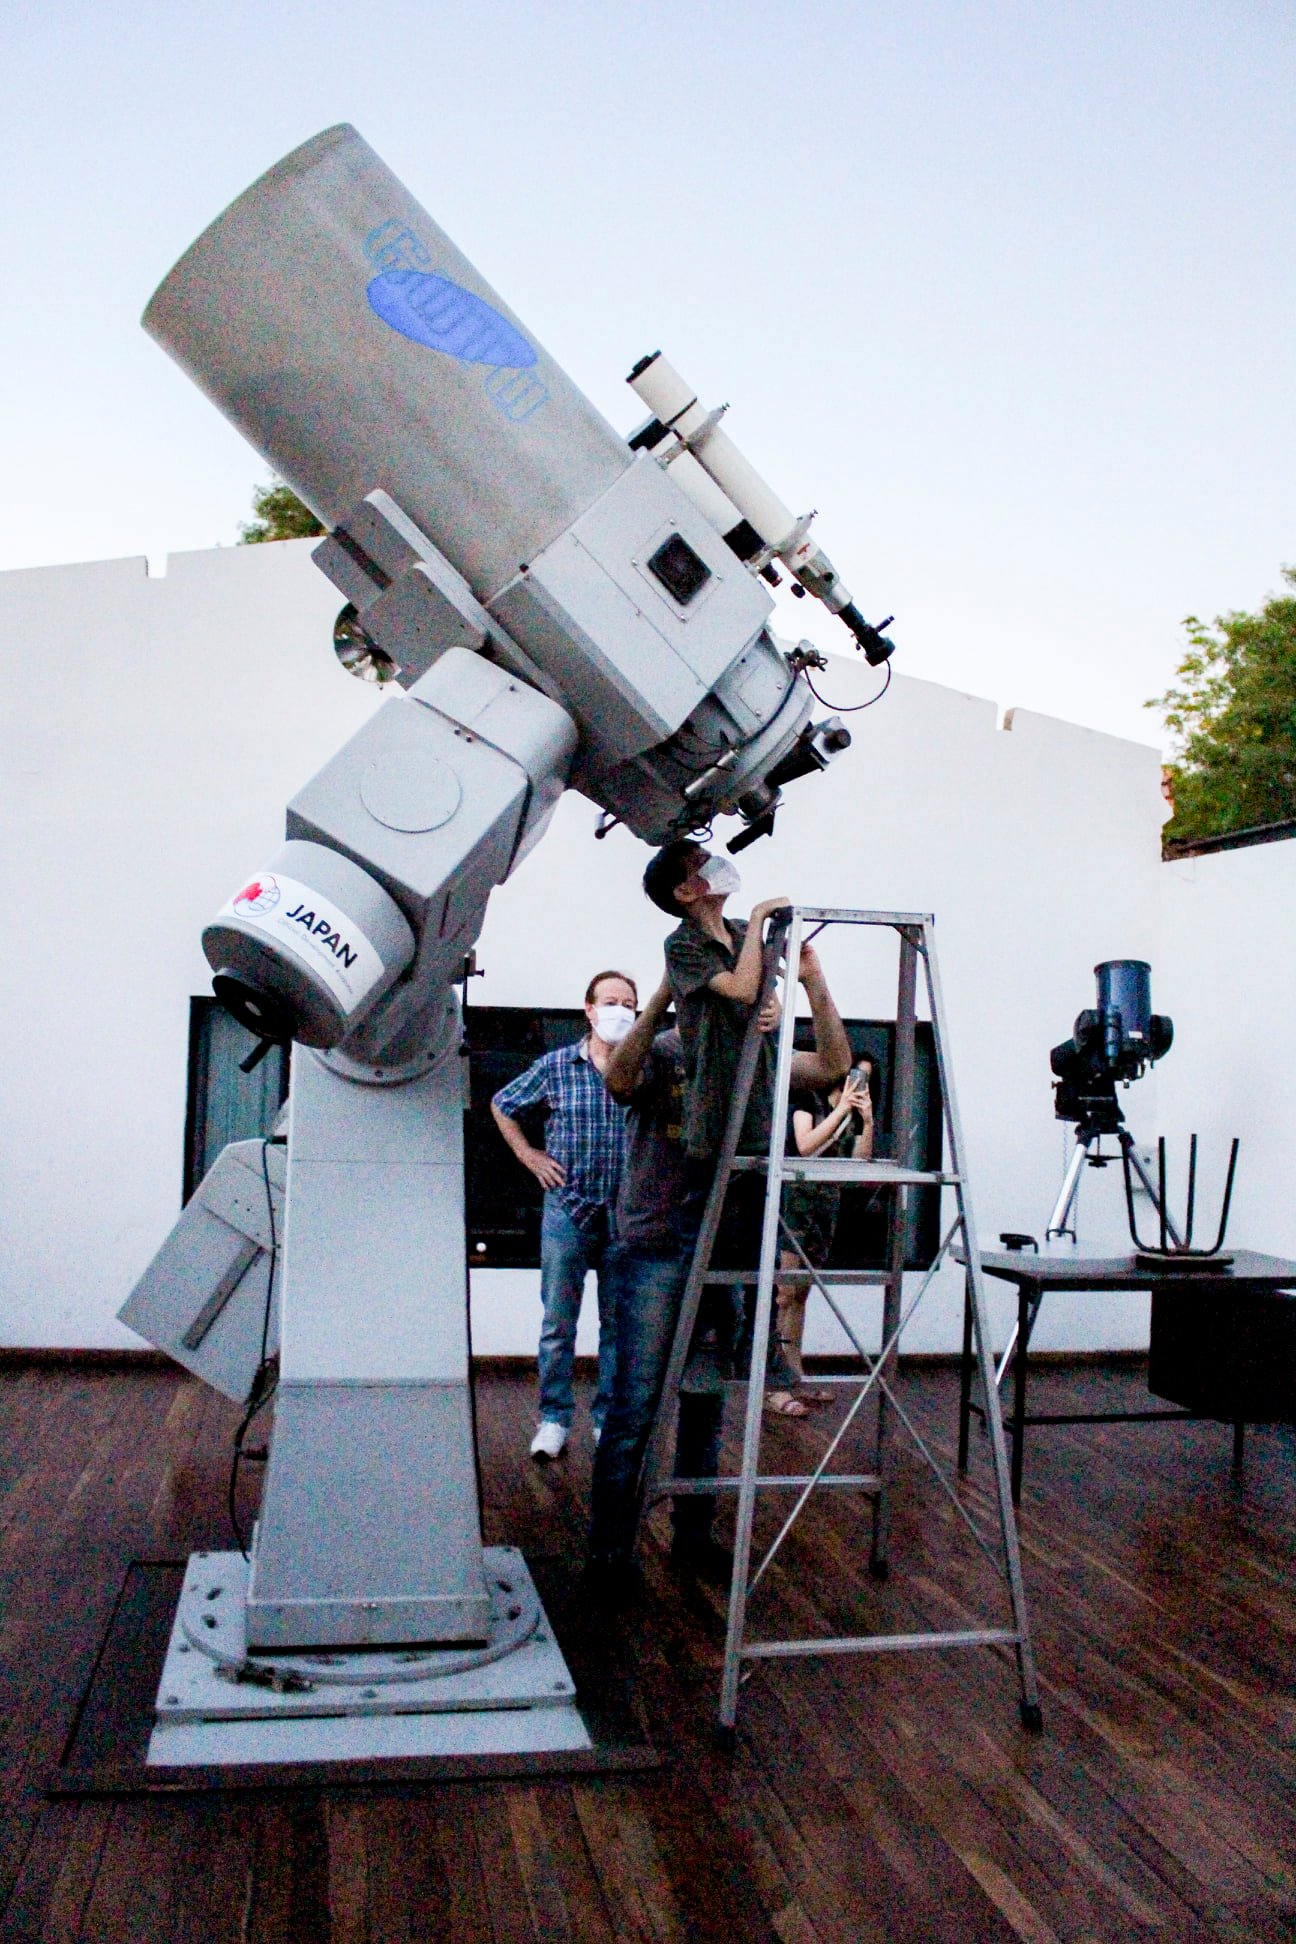
\includegraphics[width=\textwidth]{figures/obs/scope.jpg}
        \caption{Telescopio principal del observatorio.}
    \end{subfigure}
    \caption{Contexto instrumental del Observatorio Astronómico ``Prof. Alexis Troche Boggino''. La figura documenta (a) la sala de control empleada para supervisión y operación, y (b) el telescopio principal disponible en el entorno de trabajo. \textbf{Fuente:} Elaboración propia.}
    \label{fig:observatorio-alexis-troche}
\end{figure}

Las observaciones terrestres están inevitablemente afectadas por artefactos atmosféricos. Entre ellos se cuentan el \textit{seeing}, la nubosidad, el polvo sobre la óptica y la oclusión por aves o aeronaves. Estos factores producen desenfoque, distorsión y pérdidas parciales de información, y constituyen una de las principales razones por las que el análisis automático en observatorios terrestres resulta más desafiante que en imágenes espaciales. Esta observación es especialmente importante para una tesis como la presente, ya que justifica decisiones de preprocesamiento, selección de cuadros e incluso de diseño de modelos robustos frente a degradaciones no ideales.

\subsection{Observatorios espaciales y complementariedad instrumental}

La discusión de observatorios terrestres se complementa con la de observatorios espaciales. Las misiones en espacio permiten superar limitaciones atmosféricas y acceder a observaciones continuas, multiespectrales y de alta estabilidad. Entre las plataformas destacadas se encuentran SDO, SOHO, IRIS y STEREO. Estas misiones incorporan sensores capaces de observar el Sol en visible, EUV y otras longitudes de onda, así como de producir magnetogramas y reconstrucciones del campo magnético solar \citep{scherrer2012hmi,bobra2014sharp}.

\begin{figure}[H]
  \centering
  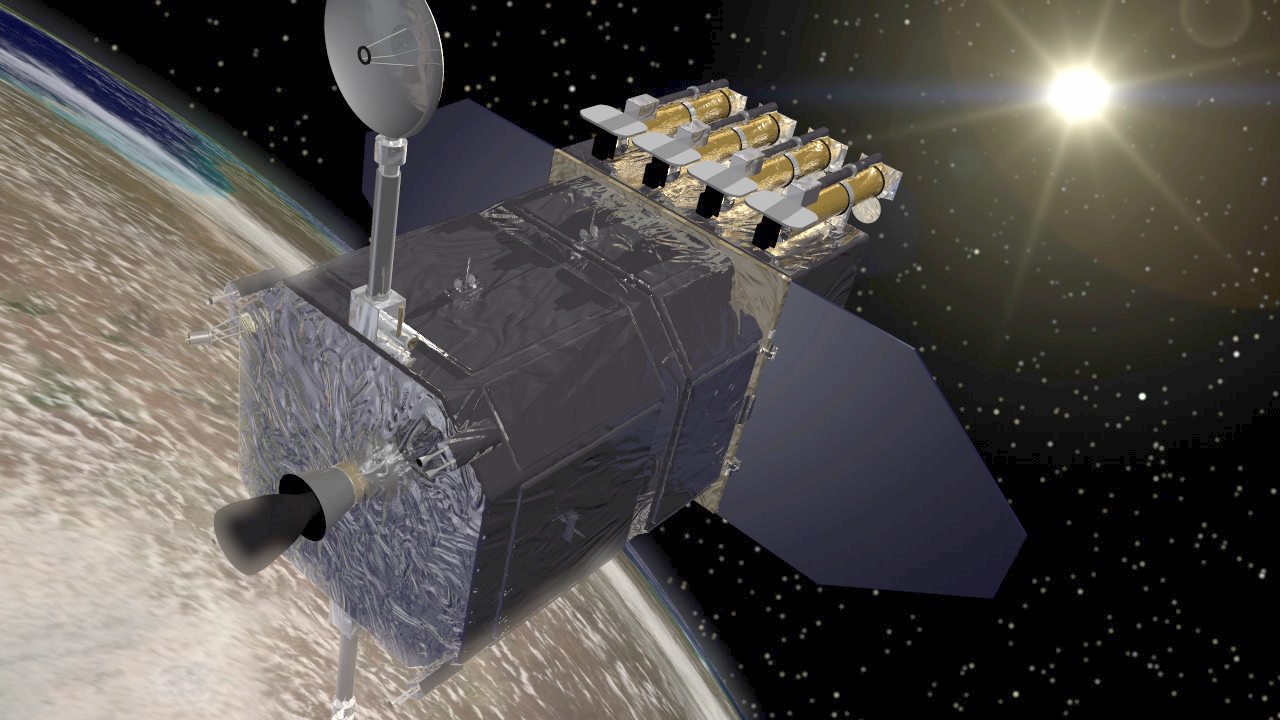
\includegraphics[width=0.78\textwidth]{figures/obs/sdo.jpg}
  \caption{Representación artística de la nave Solar Dynamics Observatory (SDO) desplegada en órbita. \textbf{Fuente:} NASA, \textit{Artist's rendition of the deployed SDO spacecraft}.}
  \label{fig:sdo-spacecraft}
\end{figure}

Para esta tesis, la importancia de tales observatorios no radica solamente en su valor científico intrínseco, sino también en su papel para la adquisición de bases de datos para entrenamiento, validación y contraste. La integración entre observaciones terrestres y espaciales amplía la capacidad de modelado del sistema solar atmosférico y habilita enfoques híbridos en los que catálogos, imágenes sinóticas y productos derivados se complementan entre sí.

\subsection{Clasificaciones observacionales de regiones activas}

La descripción de manchas solares se completa con las taxonomías empleadas para representar la complejidad de los grupos observados. En la práctica solar conviven dos familias de clasificación particularmente relevantes. Por un lado, la clasificación magnética de Mount Wilson describe la distribución de polaridad en una región activa \citep{hale1919magneticpolarity,noaaSRS} y se expresa operativamente en categorías como $\alpha$, $\beta$, $\gamma$, $\beta\gamma$ y sus variantes con modificador $\delta$. Esta taxonomía es especialmente útil cuando interesa relacionar complejidad magnética y potencial eruptivo \citep{noaaSRS}.

\begin{figure}[H]
  \centering
  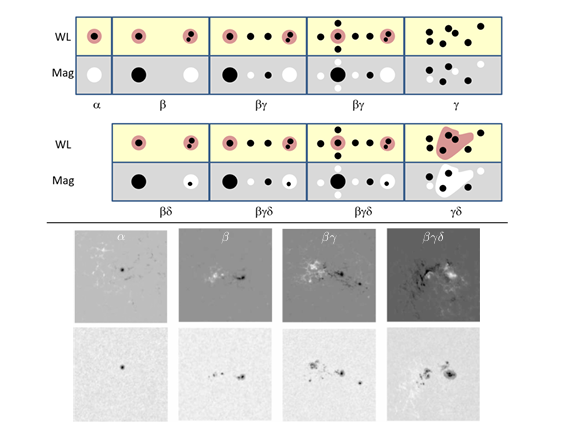
\includegraphics[width=0.65\textwidth]{figures/solar/wilson.png}
  \caption{Esquema ilustrativo de la clasificación magnética de Mount Wilson para regiones activas. La figura resume la organización de polaridades magnéticas empleada para diferenciar configuraciones simples, bipolares y complejas. \textbf{Fuente:} Adaptado de Sayez et al..}
  \label{fig:wilson-classification}
\end{figure}

Por otro lado, para observación en luz blanca y para el análisis fino de la geometría fotosférica, la clasificación Zurich--McIntosh ofrece una descripción más rica porque no se limita a indicar la polaridad magnética, sino que codifica la apariencia visible del grupo solar.

\begin{figure}[H]
  \centering
  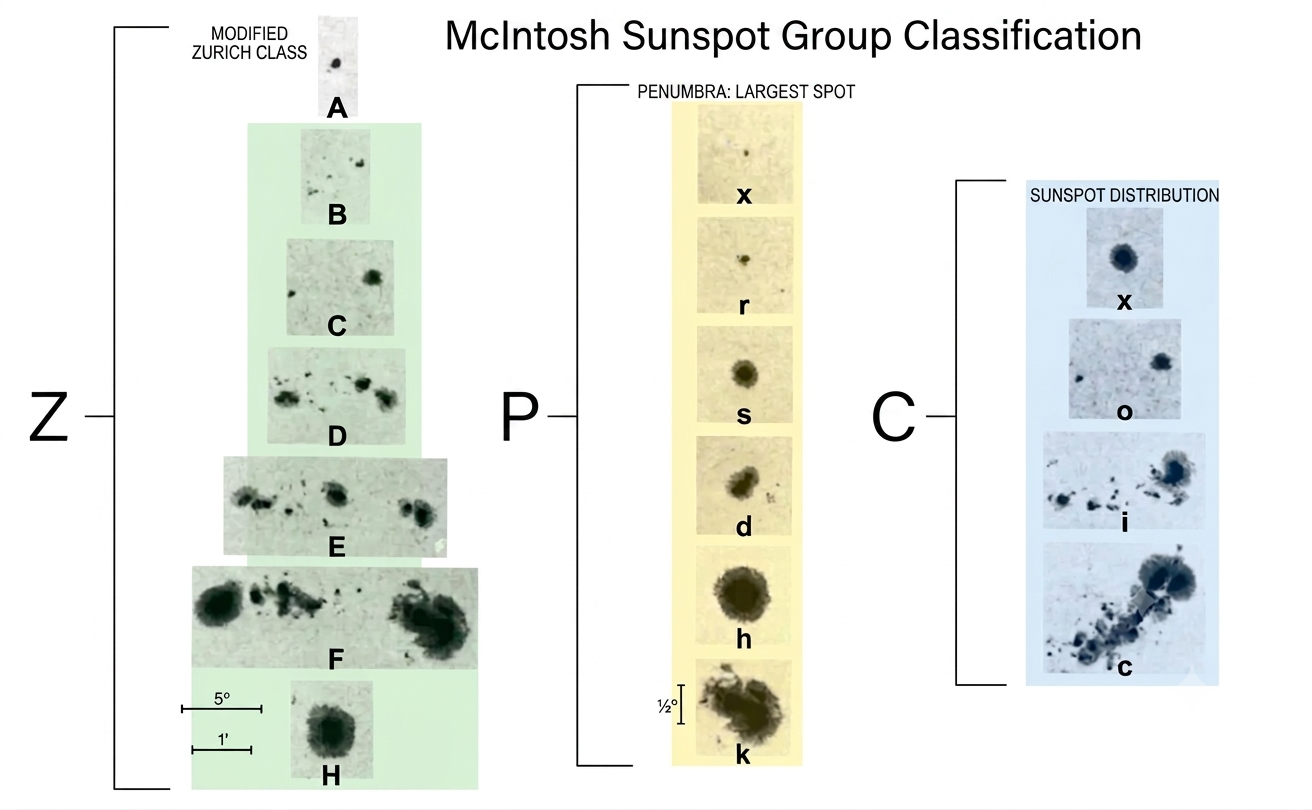
\includegraphics[width=0.62\textwidth]{figures/solar/mcintosh.png}
  \caption{Esquema general de la clasificación de McIntosh. La figura resume la combinación jerárquica de la clase Zurich, el tipo penumbral y la compactación interna del grupo solar. \textbf{Fuente:} Courtesy Patrick S. McIntosh, NOAA (1990).}
  \label{fig:mcintosh-scheme}
\end{figure}

Formalmente, estas componentes se denotan como $Z$, que describe la organización global del grupo; $P$, que caracteriza el tipo penumbral dominante; y $C$, que representa el grado de compactación interna. Esta estructura jerárquica no es solo una convención catalográfica, sino una forma compacta de codificar estado observacional, evolución estructural y relaciones geométricas visibles sobre el disco solar \citep{mcintosh1990classification,bornmann1994flarerates}.

Desde el punto de vista de esta tesis, la importancia de Zurich--McIntosh radica en que preserva semántica observacional y, al mismo tiempo, puede formularse como un problema apto para inferencia automática. Aunque la taxonomía completa puede expresarse como 60 combinaciones operativas, su interés principal no está en la enumeración exhaustiva de etiquetas, sino en la lógica jerárquica que conecta morfología global, penumbra y compactación. Precisamente por ello resulta una base adecuada para modelos de clasificación estructurada \citep{mcintosh1990classification,zhou2023mcintosh,deng2025mcintosh}.

\subsection{Cámaras para observación solar}

La discusión instrumental debe descender desde el nivel del observatorio hasta el nivel de los sensores concretos. Las cámaras constituyen el elemento que transforma la radiación proveniente del Sol en una señal digital utilizable por algoritmos de procesamiento, y por ello condicionan de manera directa la resolución espacial, la profundidad radiométrica, la cadencia temporal y la estabilidad global de la observación. En el caso de Observatorios como el USET, puede reconocerse una transición desde una práctica histórica basada en observación visual y dibujos a adquisición digital sostenida por cámaras CCD y actualmente a cámaras CMOS. Esta evolución muestra que el cambio de sensor no solo mejora la operatividad del sistema, sino que redefine la calidad y la naturaleza de los datos disponibles para el análisis.

Desde el punto de vista tecnológico, la distinción clásica entre CCD y CMOS sigue siendo importante para comprender la evolución reciente de la instrumentación astronómica. En un CCD, la carga fotoeléctrica generada en los píxeles se transfiere de manera secuencial hacia un número reducido de nodos de lectura, donde finalmente se convierte en voltaje. Esta arquitectura favoreció durante mucho tiempo una excelente uniformidad de lectura y una reputación de alta calidad científica, pero también conlleva mayor complejidad de transferencia de carga, mayor consumo energético y, en general, menores velocidades de lectura. En un CMOS, por el contrario, la conversión carga--voltaje se realiza localmente en cada píxel o en regiones muy próximas a él, lo que permite lecturas más rápidas, diseños más compactos y menor demanda energética \citep{janesick2001scientific,fossum1997cmos,zwoASI174Manual2025}.

\begin{figure}[H]
    \centering
    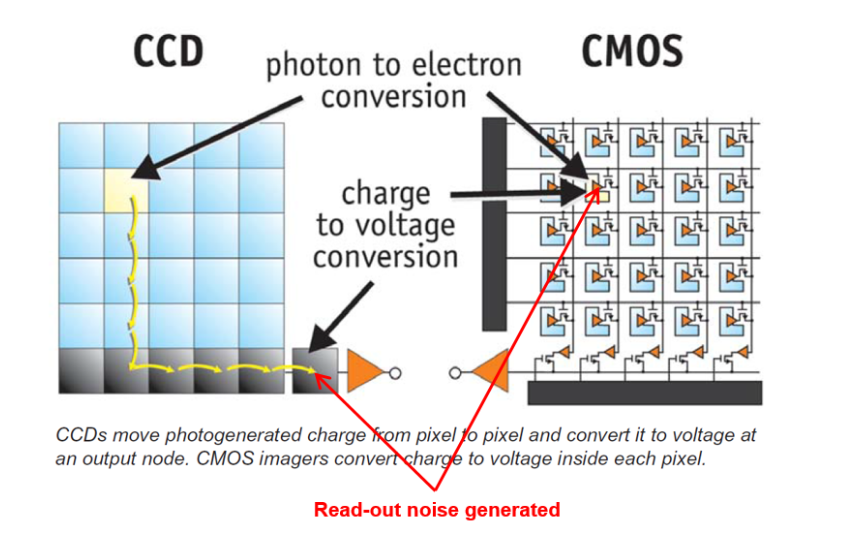
\includegraphics[width=0.78\textwidth]{figures/ml/yolo_label.png}
    \caption{Esquema conceptual de lectura en sensores CCD y CMOS. En el CCD, la carga fotoeléctrica se desplaza píxel a píxel hasta un nodo común de salida, mientras que en el CMOS la conversión carga--voltaje ocurre de forma local en cada píxel o en su vecindad inmediata. \textbf{Fuente:} Adaptado de Stefano Meroli, CERN.}
    \label{fig:ccd-cmos-readout}
\end{figure}

La diferencia entre ambas arquitecturas también tiene implicancias observacionales concretas. La literatura sobre sensores científicos indica que, en sensores CCD, el \textit{binning} puede mejorar de manera muy significativa la relación señal--ruido cuando varias cargas se suman antes de una única lectura, mientras que en CMOS el beneficio no escala de la misma manera porque el ruido de lectura se aplica a cada píxel durante la conversión local \citep{janesick2001scientific,fossum1997cmos}. Del mismo modo, la literatura técnica destaca que los CCD pueden presentar \textit{blooming} cuando una sobrecarga en un píxel se derrama hacia registros vecinos, mientras que los CMOS son intrínsecamente menos susceptibles a este fenómeno al evitar registros extensos de transferencia de carga \citep{janesick2001scientific,fossum1997cmos}. Estas diferencias no implican que una tecnología sea universalmente superior a la otra, pero sí explican por qué cada arquitectura ofrece ventajas distintas según el régimen de observación.

En astrofotografía y observación solar contemporánea, la tendencia general se ha desplazado de forma marcada hacia sensores CMOS. Esta transición se explica por la combinación de menor costo de fabricación, menor consumo, altas tasas de cuadro, ruido de lectura cada vez más competitivo y una mejora sostenida de la sensibilidad cuántica. Incluso en ámbitos donde durante años los CCD dominaron por su calidad científica, la brecha de desempeño se ha reducido de manera sustancial, y en múltiples aplicaciones los CMOS actuales ya igualan o superan prestaciones tradicionalmente asociadas a CCD astronómicos \citep{janesick2001scientific,fossum1997cmos}. Para sistemas locales de observación solar, donde interesan portabilidad, cadencia elevada y facilidad de integración con procesamiento en tiempo real, esta tendencia resulta especialmente relevante.


\begin{figure}[H]
    \centering
    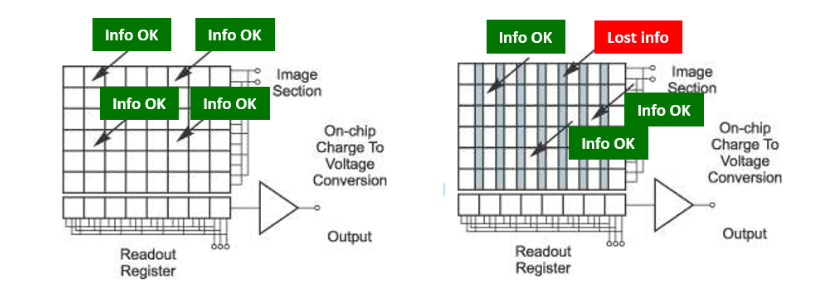
\includegraphics[width=0.86\textwidth]{figures/ml/yolo_box.png}
    \caption{Esquema conceptual del efecto de lectura sobre la integridad de la información en sensores con conversión distribuida. \textbf{Fuente:} Adaptado de Stefano Meroli, CERN.}
    \label{fig:ccd-cmos-info}
\end{figure}

Las Figuras \ref{fig:ccd-cmos-readout} y \ref{fig:ccd-cmos-info} resumen visualmente esta diferencia de arquitectura. La primera destaca el contraste entre transferencia serial de carga en CCD y conversión local en CMOS, mientras que la segunda ayuda a interpretar por qué la organización del trayecto de lectura puede impactar la preservación de información útil y la generación de ruido durante la adquisición.

\section{Estado del Arte}

En esta tesis, el estado del arte se organiza a partir de una limitación observada en el ecosistema tecnológico disponible: existen soluciones comerciales avanzadas para asistir la adquisición y operación de equipos de astrofotografía, así como investigaciones recientes para detectar, agrupar, clasificar y predecir la actividad asociada a manchas solares; sin embargo, no se identifican ecosistemas comerciales de observación astrofotográfica que integren de forma específica todas las etapas requeridas para este trabajo, desde la adquisición local de imágenes solares hasta el análisis morfológico y la generación de indicadores predictivos basados en modelos computacionales. Por ello, la revisión se presenta en subsecciones complementarias que cubren, primero, dispositivos comerciales de adquisición asistida y, luego, contribuciones recientes sobre análisis automático de manchas solares.

En el plano algorítmico, el problema automático de análisis de manchas solares se organiza en dos ejes complementarios: el agrupamiento y clasificación morfológica, y el análisis predictivo de la actividad de manchas solares (Número de manchas solares y distribución latitudinal). Esta descomposición no es arbitraria, sino que responde a la propia lógica observacional del problema. La clasificación Zurich--McIntosh se aplica sobre el grupo solar como unidad de análisis y no sobre manchas aisladas; por ello, antes de clasificar, es necesario detectar y asociar correctamente las manchas que pertenecen a una misma estructura activa \citep{sayez2023sunscc}. De forma complementaria, la interpretación temporal de esos grupos se inserta en la modulación de gran escala impuesta por el ciclo solar.

\subsection{Dispositivos comerciales de adquisición de imágenes asistida}

Los dispositivos comerciales de adquisición asistida para astrofotografía han evolucionado hacia unidades compactas que combinan control de cámaras, monturas, enfocadores, ruedas portafiltros, alimentación eléctrica y conectividad inalámbrica. Su objetivo principal es reducir la complejidad operativa de una sesión de captura, centralizando el control instrumental en una aplicación móvil o en una interfaz remota. La Figura~\ref{fig:hw-art-state-commercial} muestra tres ejemplos representativos de esta tendencia: ZWO ASIAIR, PrimaLuceLab EAGLE6 y StellarMate Pro.

\begin{figure}[H]
    \centering
    \begin{subfigure}[t]{0.31\textwidth}
        \centering
        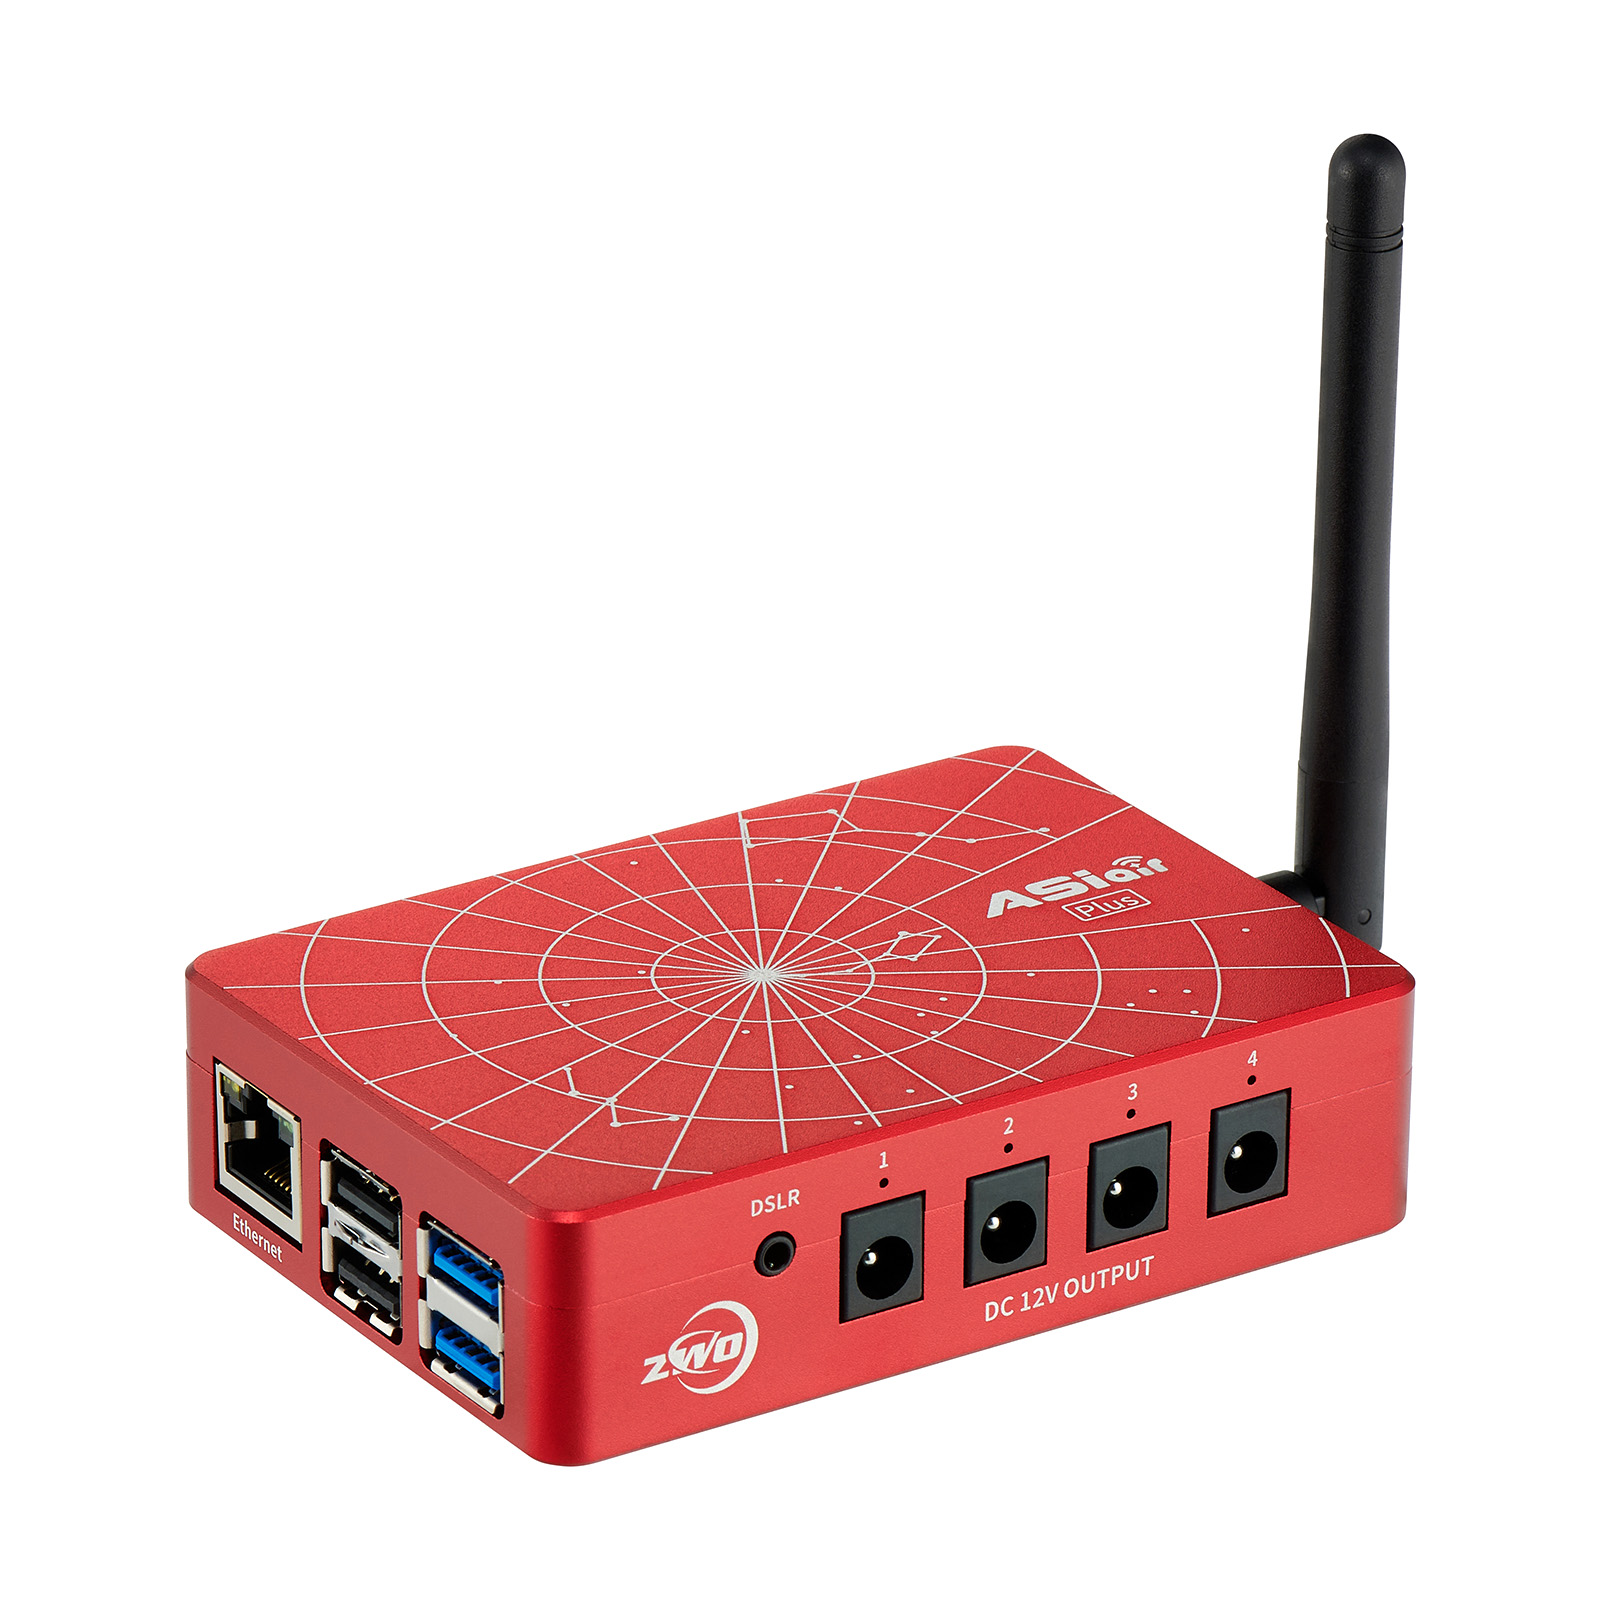
\includegraphics[width=\textwidth]{figures/hw_art_state/zwo_asiair.jpg}
        \caption{ZWO ASIAIR.}
    \end{subfigure}
    \hfill
    \begin{subfigure}[t]{0.31\textwidth}
        \centering
        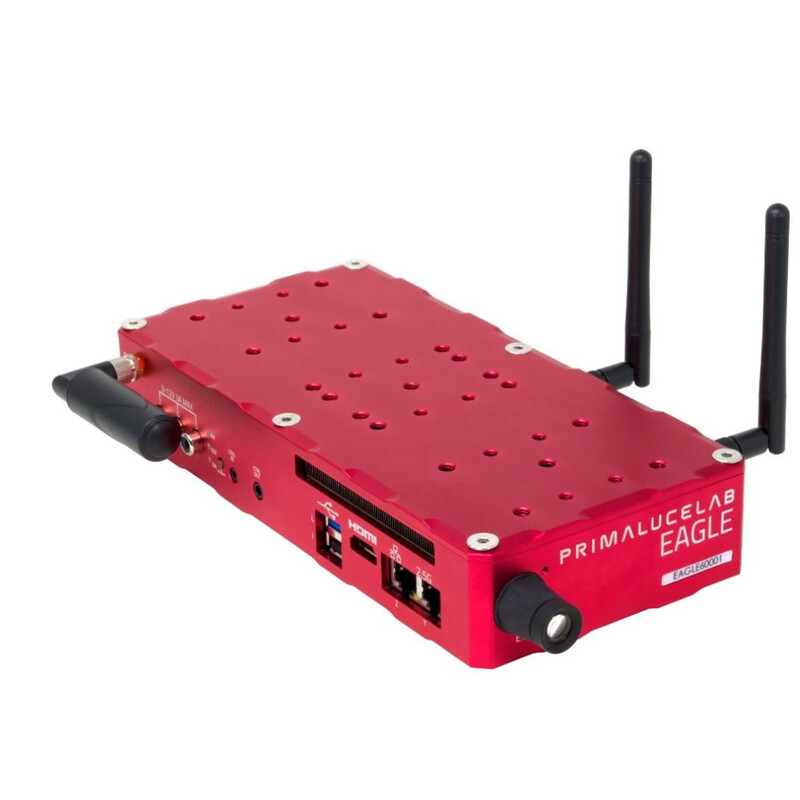
\includegraphics[width=\textwidth]{figures/hw_art_state/primaLuceLab-Eagle6.jpg}
        \caption{PrimaLuceLab EAGLE6.}
    \end{subfigure}
    \hfill
    \begin{subfigure}[t]{0.31\textwidth}
        \centering
        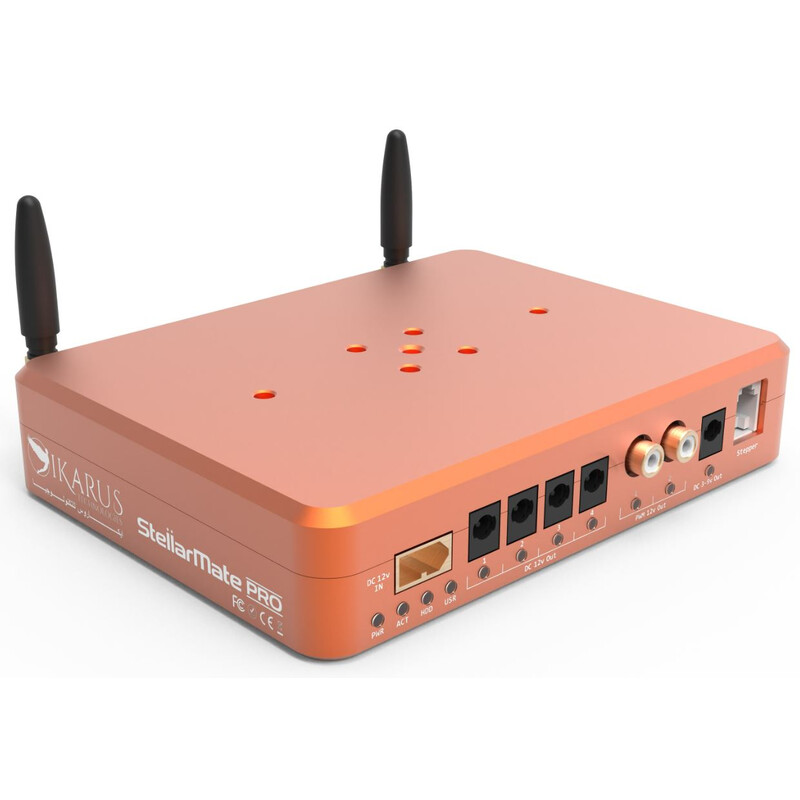
\includegraphics[width=\textwidth]{figures/hw_art_state/stellar_mate-pro-8GB-128GB.jpg}
        \caption{StellarMate Pro.}
    \end{subfigure}
    \caption{Dispositivos comerciales de adquisición asistida empleados como referencia del estado del arte instrumental en astrofotografía. \textbf{Fuente:} páginas oficiales de ZWO, PrimaLuceLab y StellarMate.}
    \label{fig:hw-art-state-commercial}
\end{figure}

ZWO ASIAIR representa una aproximación cerrada y altamente integrada alrededor del ecosistema ZWO. En su versión Plus de 256~GB se comercializa alrededor de US\$349, incorpora 4~GB de RAM DDR4, almacenamiento eMMC de 32~GB o 256~GB, red Gigabit Ethernet, WiFi de doble banda y cuatro salidas de 12~V con capacidad máxima conjunta de 5~A \citep{zwoASIAIR2026,bhASIairPlus2026}. Su principal fortaleza es la simplicidad de uso y la integración directa con cámaras, monturas y accesorios compatibles, aunque dicha integración tiende a privilegiar un entorno de hardware específico.

PrimaLuceLab EAGLE6 adopta una estrategia más cercana a una computadora industrial para telescopios. Su precio de referencia es aproximadamente US\$1595 e integra Windows 11 Enterprise, procesador Intel Celeron J6412, 8~GB de memoria DDR4, almacenamiento NVMe industrial de 128~GB, conectividad WiFi 6E, GPS, diez puertos USB y siete salidas de alimentación de 12~V, además de sensores auxiliares para monitoreo de cielo, inclinación y movimiento \citep{primaluceEagle62026,primaluceEagle6USA2026}. Por estas características, se orienta a configuraciones de observatorio o montajes de mayor complejidad, donde la distribución de energía y la gestión remota son tan importantes como la captura de imágenes.

StellarMate Pro, por su parte, se presenta como un controlador de clase observatorio basado en tecnologías abiertas. La versión de 128~GB se ofrece alrededor de US\$599 e incorpora 8~GB de RAM, SSD de 128~GB, procesador Broadcom BCM2711, cuatro puertos USB 3.0, dos puertos USB 2.0, cuatro salidas de 12~V, dos salidas para calentadores antirocío, una salida variable de 3--9~V, conectividad HDMI/Ethernet/GPS/WiFi y sistema StellarMate OS precargado \citep{stellarmatePro2026}. A diferencia de soluciones más cerradas, su propuesta enfatiza compatibilidad con distintos fabricantes mediante el ecosistema INDI/KStars/Ekos, lo que resulta atractivo para configuraciones heterogéneas.

La Tabla~\ref{tab:dispositivos-adquisicion-comerciales} resume las características técnicas más relevantes para comparar estos dispositivos como plataformas de adquisición asistida. Los precios deben interpretarse como valores comerciales de referencia sujetos a variación por distribuidor, impuestos, disponibilidad y configuración seleccionada.

\begin{table}[H]
\centering
\caption{Exploración de dispositivos comerciales de adquisición asistida para astrofotografía. Los precios son referenciales y pueden variar según configuración, distribuidor y fecha de consulta. \textbf{Fuente:} Elaboración propia a partir de páginas oficiales y distribuidores autorizados \citep{zwoASIAIR2026,bhASIairPlus2026,primaluceEagle62026,primaluceEagle6USA2026,stellarmatePro2026}.}
\label{tab:dispositivos-adquisicion-comerciales}
\uniformtablestyle
\begin{tabularx}{\textwidth}{>{\raggedright\arraybackslash}p{3.35cm} >{\raggedright\arraybackslash}p{3.15cm} >{\centering\arraybackslash}p{1.45cm} X}
\toprule
\textbf{Fabricante / modelo} & \textbf{Característica técnica} & \textbf{Precio ref.} & \textbf{Observaciones} \\
\midrule
ZWO ASIAIR Plus 256~GB & 4~GB DDR4; 32/256~GB eMMC; Ethernet; WiFi 2.4/5~GHz & US\$349 & Se destaca por su integración directa con el ecosistema ZWO y por operar desde la aplicación ASIAIR en teléfono inteligente o tableta. \\
PrimaLuceLab EAGLE6 & 8~GB DDR4; 128~GB NVMe SSD; WiFi 6E; Ethernet 2.5~Gb; GPS; Windows 11 Enterprise & US\$1595 & Se destaca por su enfoque de computadora industrial para telescopios, con sensores auxiliares y gestión avanzada de observatorio. \\
StellarMate Pro 128~GB & 8~GB LPDDR4; 128~GB SSD; WiFi 5; Bluetooth 5.0; Ethernet; GPS; StellarMate OS & US\$599 & Se destaca por su compatibilidad con equipos heterogéneos mediante INDI/KStars/Ekos y por una propuesta basada en tecnologías abiertas. \\
\bottomrule
\end{tabularx}
\end{table}

Estos productos evidencian que el mercado ya ofrece plataformas robustas para automatizar la adquisición y operación instrumental. No obstante, su alcance se concentra principalmente en la captura astrofotográfica, el control de periféricos y el soporte a flujos de observación general. En contraste, el objetivo de esta tesis requiere integrar adquisición solar en luz blanca, preprocesamiento local, detección y agrupamiento de manchas, clasificación Zurich--McIntosh y análisis predictivo de la actividad solar dentro de un flujo específico. Esta brecha justifica revisar por separado tanto el estado del arte instrumental como los avances recientes en análisis automático de manchas solares.

\subsection{Agrupamiento y clasificación de manchas solares}

Las investigaciones recientes \cite{sayez2023sunscc} sugieren que las estrategias más consistentes no abordan el problema como una clasificación directa de regiones aisladas, sino como una arquitectura modular en la que primeramente se detectan y agrupan manchas individuales, y luego se clasifica el grupo solar resultante. 
\begin{figure}[H]
    \centering
    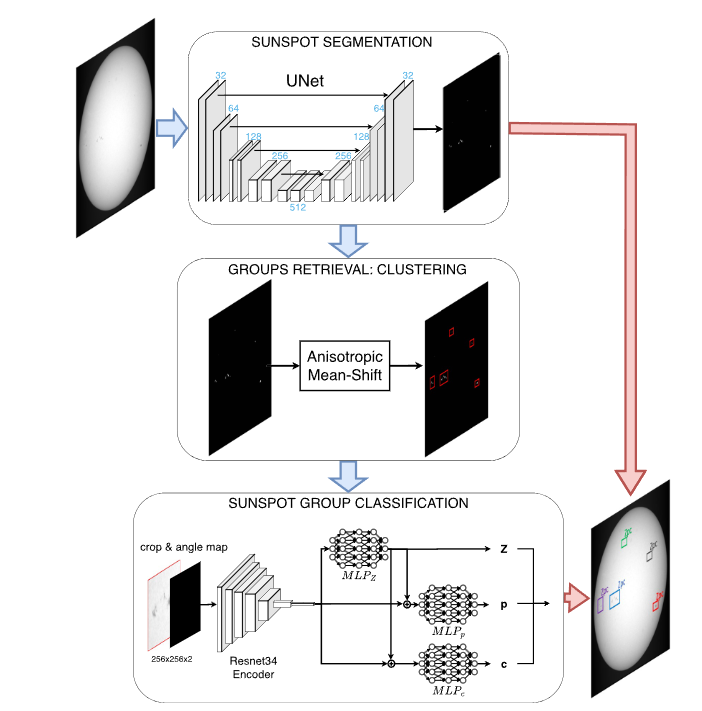
\includegraphics[width=0.5\textwidth]{figures/ml/yolo_train.png}
    \caption{Esquema del enfoque modular presentado por Sayez et al. \cite{sayez2023sunscc}, donde el flujo de procesamiento se modula en segmentación, agrupamiento y clasificación de manchas solares. \textbf{Fuente:} 
    Adaptado de Sayez et al..}
    \label{fig:sunscc_pipeline_stateoftheart}
\end{figure}

Este enfoque refleja mejor la lógica observacional de la taxonomía Zurich--McIntosh y, además, es el que mejores resultados comparativos reporta hasta la fecha entre los trabajos de referencia considerados en esta tesis Sayez et al. \citep{sayez2023sunscc,deng2025mcintosh}.

En consecuencia, el hilo conductor de este apartado consiste en examinar, primero, cómo se construye la unidad observacional relevante o grupo solar, y seguidamente, cómo dicha unidad se clasifica morfológicamente de forma automática.


\subsubsection{Agrupamiento de manchas solares}

La detección precisa de las manchas solares es fundamental para la construcción de índices de actividad solar (Número de Wolf; \citep{clette2007wolf}), y constituye además el punto de partida para cualquier procedimiento automático de agrupamiento y clasificación \citep{clette2007wolf,sayez2023sunscc}. Sin embargo, la delineación de manchas no es un problema completamente objetivo. Distintos observadores pueden discrepar en los bordes o en la separación de estructuras cercanas; además, las manchas presentan formas irregulares, contraste variable con la fotosfera y diferentes niveles de degradación cuando las imágenes provienen de observatorios terrestres.

En este contexto, la literatura reporta dos grandes familias de métodos de detección automática. Por un lado, los métodos basados en regiones utilizan umbralado, histogramas de intensidad con enfoques bayesianos o procedimientos de crecimiento de regiones para separar las manchas del fondo fotosférico a partir de propiedades radiométricas y de conectividad local \citep{pettauer1997sunspots,steinegger1998thresholds,turmon2002pattern,murakozy2022asymmetries}. Por otro lado, los métodos basados en bordes se concentran en las discontinuidades de la imagen y en la localización de contornos, a menudo complementados con operaciones de morfología matemática sobre imágenes de continuo \citep{zharkov2005automated,scherrer1995mdi,curto2008morphology,watson2009wilson}.

Una referencia importante en esta comparación es el trabajo de Carvalho et al. \citep{carvalho2020comparison}, donde muestran que los enfoques basados en morfología matemática tienden a comportarse mejor que los métodos puramente basados en intensidad. Además, requieren menos preprocesamiento para atenuar efectos atmosféricos y corregir el oscurecimiento hacia el limbo. No obstante, estos métodos siguen dependiendo en gran medida de elecciones heurísticas, como el tamaño de los operadores morfológicos o la fijación de umbrales, lo que limita su robustez frente a variaciones instrumentales y observacionales.

La literatura ha explorado diversas estrategias para resolver este problema. Nguyen et al. \citep{nguyen2004learning} evaluaron algoritmos jerárquicos y un esquema simple de \textit{k-means}, mostrando que este último resulta poco práctico cuando el número de grupos presentes en una observación no es conocido de antemano. Del mismo modo, los métodos jerárquicos dependen fuertemente del criterio de parada. En un trabajo posterior, los mismos autores compararon estas estrategias con DBSCAN y reportaron un comportamiento ligeramente mejor de los enfoques basados en densidad \citep{nguyen2006hybrid,ester1996dbscan}.

Dentro de este panorama, el algoritmo \textit{mean-shift} resulta especialmente atractivo porque permite localizar máximos locales de densidad en el espacio de observación e incorporar, de manera natural, conocimiento previo sobre la elongación anisotrópica de los clústeres. Esta propiedad lo vuelve particularmente adecuado para el problema solar, ya que los grupos de manchas muestran una organización longitudinal dominante. Por ello, la revisión más reciente considera que el agrupamiento debe diseñarse como una etapa independiente entre la detección de manchas y la clasificación del grupo, y no como una simple extensión geométrica de la segmentación \citep{comaniciu2002mean,sayez2023sunscc}.

En paralelo a estos métodos geométricos, los detectores de la familia YOLO han adquirido relevancia por formular la detección como un problema integrado de estimación de clases y cajas delimitadoras, con tiempos de inferencia compatibles con aplicaciones de baja latencia. Frente a modelos previos de la misma familia, YOLO26 enfatiza una arquitectura más simple y directamente desplegable: adopta una formulación nativa \textit{end-to-end}, reduce la dependencia de etapas externas de posprocesamiento y elimina la supresión no máxima (NMS) como requisito operativo. Esta diferencia es relevante porque, en variantes tradicionales, la salida del modelo suele requerir un procedimiento posterior para filtrar predicciones redundantes; al incorporar dicha resolución dentro del propio esquema de inferencia, se reduce la complejidad operacional, se simplifica la exportación y se facilita la ejecución en dispositivos de borde.

La propuesta también se distancia de versiones anteriores al retirar la formulación DFL, que aunque resulta útil para refinar la regresión de cajas, puede introducir complejidad adicional en la exportación y reducir compatibilidad con ciertos aceleradores o entornos de bajo consumo. A esto se suman innovaciones de entrenamiento, como el optimizador MuSGD y mejoras de pérdida orientadas a objetos pequeños, además de módulos específicos para segmentación, pose y detección orientada. En conjunto, estas decisiones apuntan a mantener precisión competitiva con menor costo de integración, y la documentación técnica reporta mejoras de velocidad de inferencia en CPU de hasta el 43\% respecto de configuraciones anteriores bajo sus condiciones de evaluación \citep{ultralyticsYOLO26}. En el contexto de esta tesis, esta orientación resulta pertinente porque el detector debe operar sobre imágenes solares completas, localizar estructuras de bajo tamaño relativo y conservar viabilidad computacional en un entorno de adquisición local.

La comparación con YOLOv8 y YOLO11 debe plantearse en función del escenario de despliegue. Ambas arquitecturas constituyen alternativas consolidadas para detección general, con disponibilidad de pesos preentrenados y desempeño robusto en bancos de prueba estándar; no obstante, su cadena de inferencia puede conservar dependencias de posprocesamiento o relaciones menos favorables entre precisión, latencia y costo de exportación cuando se prioriza ejecución en CPU o hardware embebido. Para una aplicación astronómica local, donde la inferencia debe repetirse sobre secuencias de imágenes solares y donde las manchas ocupan una fracción reducida del disco, YOLO26 ofrece una ventaja técnica al reducir la complejidad de despliegue y priorizar un equilibrio más explícito entre exactitud, velocidad y tamaño del modelo. Por ello, frente a YOLOv8 o YOLO11, su interés no se limita a una mejora de métrica aislada, sino a una adecuación más directa a sistemas de monitoreo solar ejecutados en nodos de borde.

\begin{figure}[H]
    \centering
    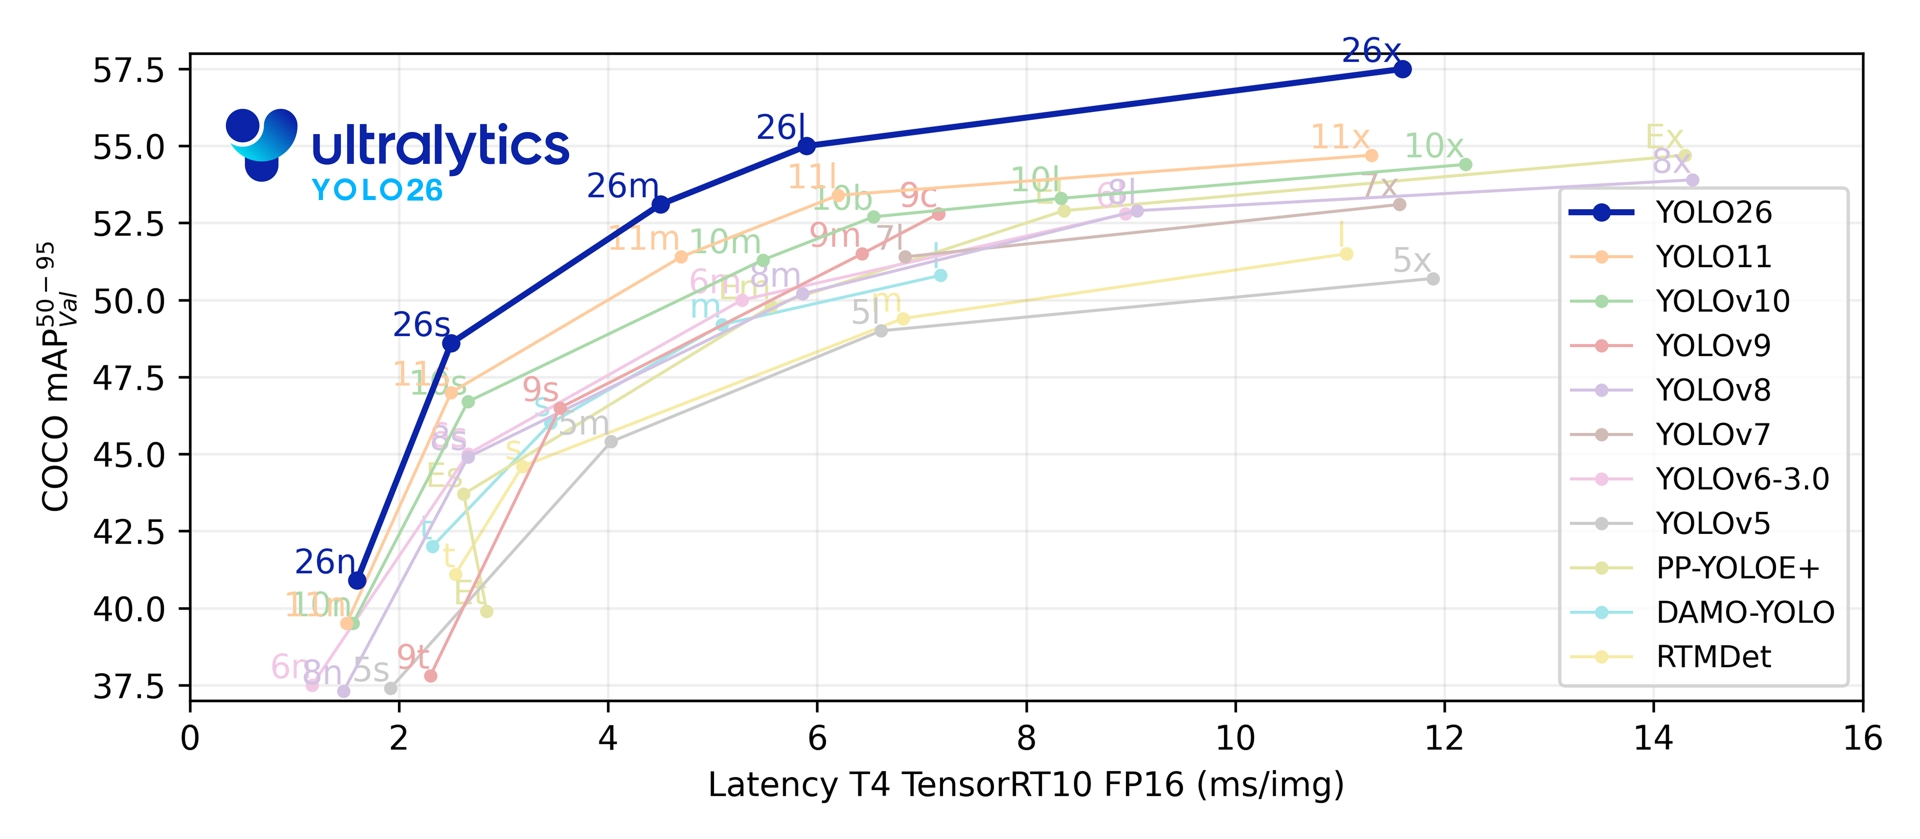
\includegraphics[width=0.92\textwidth]{figures/ml/yolo_bench.jpg}
    \caption{Comparación de desempeño de Ultralytics YOLO26 frente a modelos YOLO previos. La gráfica resume el compromiso entre precisión, velocidad y tamaño de las variantes, destacando la orientación de YOLO26 hacia inferencia eficiente y despliegue en escenarios con recursos restringidos. Adaptado de.}
    \label{fig:yolo26-benchmark}
\end{figure}

Esta discusión permite interpretar la elección de YOLO no solo como una decisión de precisión, sino como una decisión de arquitectura orientada al despliegue. Para un sistema de monitoreo solar, el detector debe localizar manchas pequeñas dentro de imágenes de disco completo, mantener tiempos de respuesta compatibles con adquisición continua y, al mismo tiempo, evitar una carga computacional excesiva en hardware local. En ese marco, la comparación de variantes resulta útil para evaluar el compromiso entre exactitud, latencia y tamaño del modelo.

La Figura~\ref{fig:yolo26-benchmark} sintetiza precisamente este posicionamiento: YOLO26 no se presenta únicamente como una iteración de mayor precisión, sino como una familia optimizada para equilibrar desempeño y complejidad de despliegue. La variante nano, YOLO26n, es la más adecuada cuando el objetivo no es maximizar la precisión en un servidor de entrenamiento, sino sostener inferencia rápida sobre hardware restringido. Para entrada de $640\times640$ píxeles, la documentación de referencia reporta aproximadamente $2.4$ millones de parámetros y $5.4$ GFLOPs en el modelo fusionado, con una precisión COCO mAP$_{50:95}$ de $40.9$ y tiempos de inferencia CPU--ONNX del orden de decenas de milisegundos bajo el entorno de evaluación reportado \citep{ultralyticsYOLO26}. Esta escala paramétrica es importante para el problema solar: las manchas ocupan áreas relativamente pequeñas dentro del disco completo, por lo que se requiere una arquitectura capaz de conservar sensibilidad espacial sin volver inviable la ejecución local.


\subsubsection{Clasificación morfológica de grupos solares}

La segunda etapa del problema corresponde a la clasificación morfológica de los grupos solares ya delimitados. A pesar de que las reglas de clasificación están formalmente establecidas, esta tarea continúa realizándose manualmente en numerosos observatorios y sigue estando expuesta a subjetividad, sesgos entre observadores y discrepancias en la interpretación de configuraciones morfológicas cercanas.

Las primeras propuestas automáticas combinaron umbralado, reglas manuales y clasificadores poco profundos sobre imágenes de continuo y magnetogramas. Aunque estos trabajos constituyen antecedentes importantes, muchos de ellos se validaron sobre conjuntos de datos reducidos o simplificados, lo que limita la generalización de sus resultados. Más recientemente, la clasificación automática ha pasado a apoyarse en CNN, aprendizaje por transferencia y esquemas multitarea capaces de predecir las componentes de la taxonomía Zurich--McIntosh de manera más estructurada.

En este contexto, Palladino et al. \citep{palladino2022sunspot} abordan la tarea mediante detección y clasificación apoyadas en imágenes de continuo, magnetogramas y tablas SRS, observando que la confusión entre clases cercanas del componente $Z$ en particular entre D, E y F sigue siendo una de las principales dificultades del problema. Por su parte, Sayez et al. \citep{sayez2023sunscc} formulan la clasificación como un problema jerárquico, donde las componentes $Z$, $P$ y $C$ se predicen de manera dependiente y se complementan con agregación de clases y ensambles para estimar confiabilidad. Esta estrategia resulta especialmente relevante para esta tesis porque preserva la estructura semántica de la clasificación en el propio diseño del modelo.

La literatura reciente muestra además dos tendencias complementarias. Una busca mantener la taxonomía completa para conservar riqueza observacional y trazabilidad; la otra simplifica el espacio de clases o predice por componentes para estabilizar el aprendizaje en escenarios con fuerte desbalance. En esa línea, Zhou et al. \citep{zhou2023mcintosh} subrayan la necesidad de ampliar y depurar las bases de datos McIntosh, mientras que trabajos más recientes como Deng et al. \citep{deng2025mcintosh} continúan explorando arquitecturas profundas para clasificación morfológica fina.

Dentro de este escenario, ConvNeXtV2 representa una alternativa relevante frente a CNN clásicas y arquitecturas basadas exclusivamente en transformadores. Su interés proviene de modernizar una red convolucional pura con decisiones inspiradas por los avances recientes en visión: bloques residuales profundos, convoluciones de gran campo efectivo, normalización por capas, activaciones suaves y una organización por etapas que facilita transferencia de aprendizaje. La segunda versión añade una capa de \textit{Global Response Normalization} (GRN) y se co-diseña con un esquema de preentrenamiento auto-supervisado mediante \textit{Fully Convolutional Masked Autoencoder} (FCMAE), lo que mejora la competencia entre canales y la calidad de las representaciones aprendidas \citep{woo2023convnextv2}.

\begin{figure}[H]
  \centering
  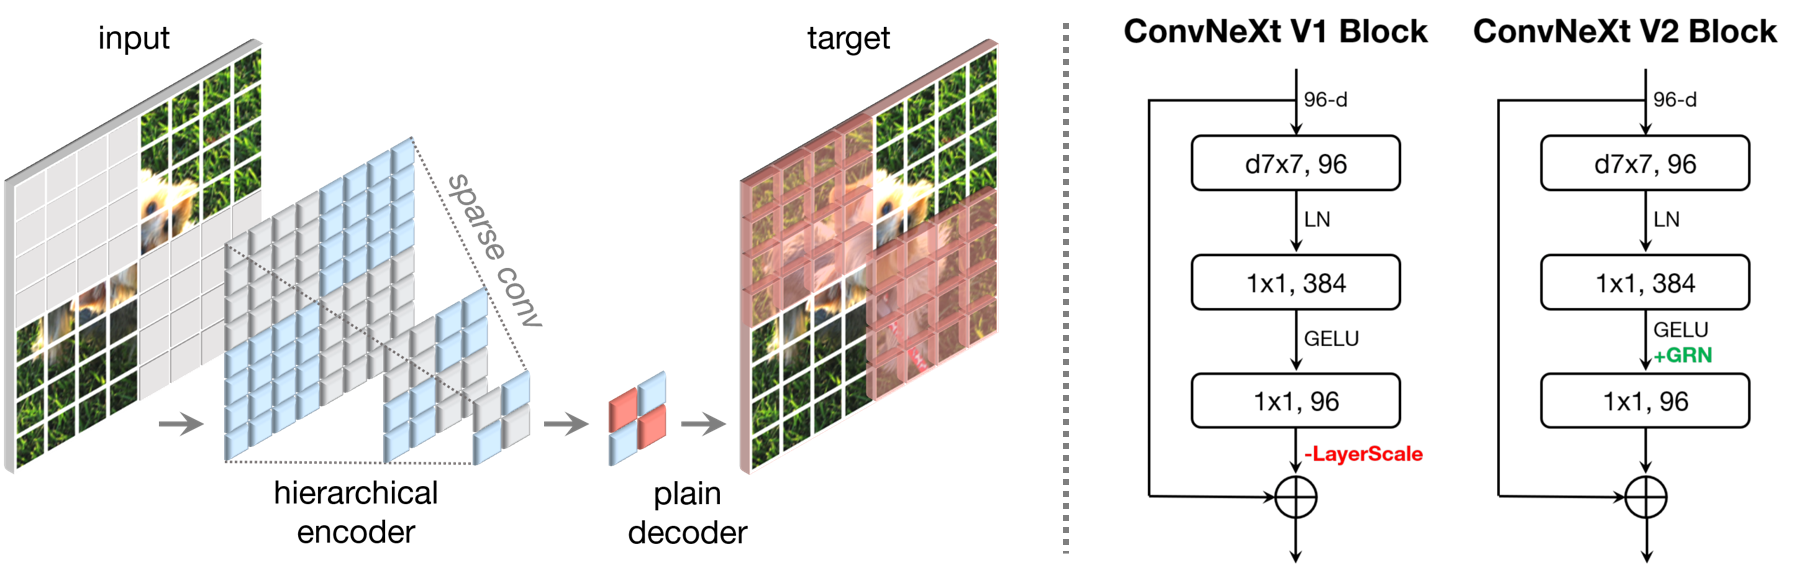
\includegraphics[width=0.82\textwidth]{figures/ml/fcmae.png}
  \caption{Esquema de preentrenamiento FCMAE empleado en ConvNeXtV2. La estrategia enmascara regiones de entrada y fuerza al codificador convolucional a reconstruir información visual faltante, favoreciendo representaciones robustas antes del ajuste supervisado. \textbf{Fuente:} Adaptado de Woo et al..}
  \label{fig:convnextv2-fcmae}
\end{figure}

El esquema de la Figura~\ref{fig:convnextv2-fcmae} es especialmente pertinente para clasificación morfológica porque desplaza parte del aprendizaje desde etiquetas discretas hacia la estructura visual de las imágenes. En un problema como Zurich--McIntosh, donde las clases pueden diferir por continuidad penumbral, compactación o distribución interna de manchas, este tipo de preentrenamiento resulta útil para inicializar extractores de características sensibles a textura, contorno y organización espacial del grupo solar.

\begin{figure}[H]
  \centering
  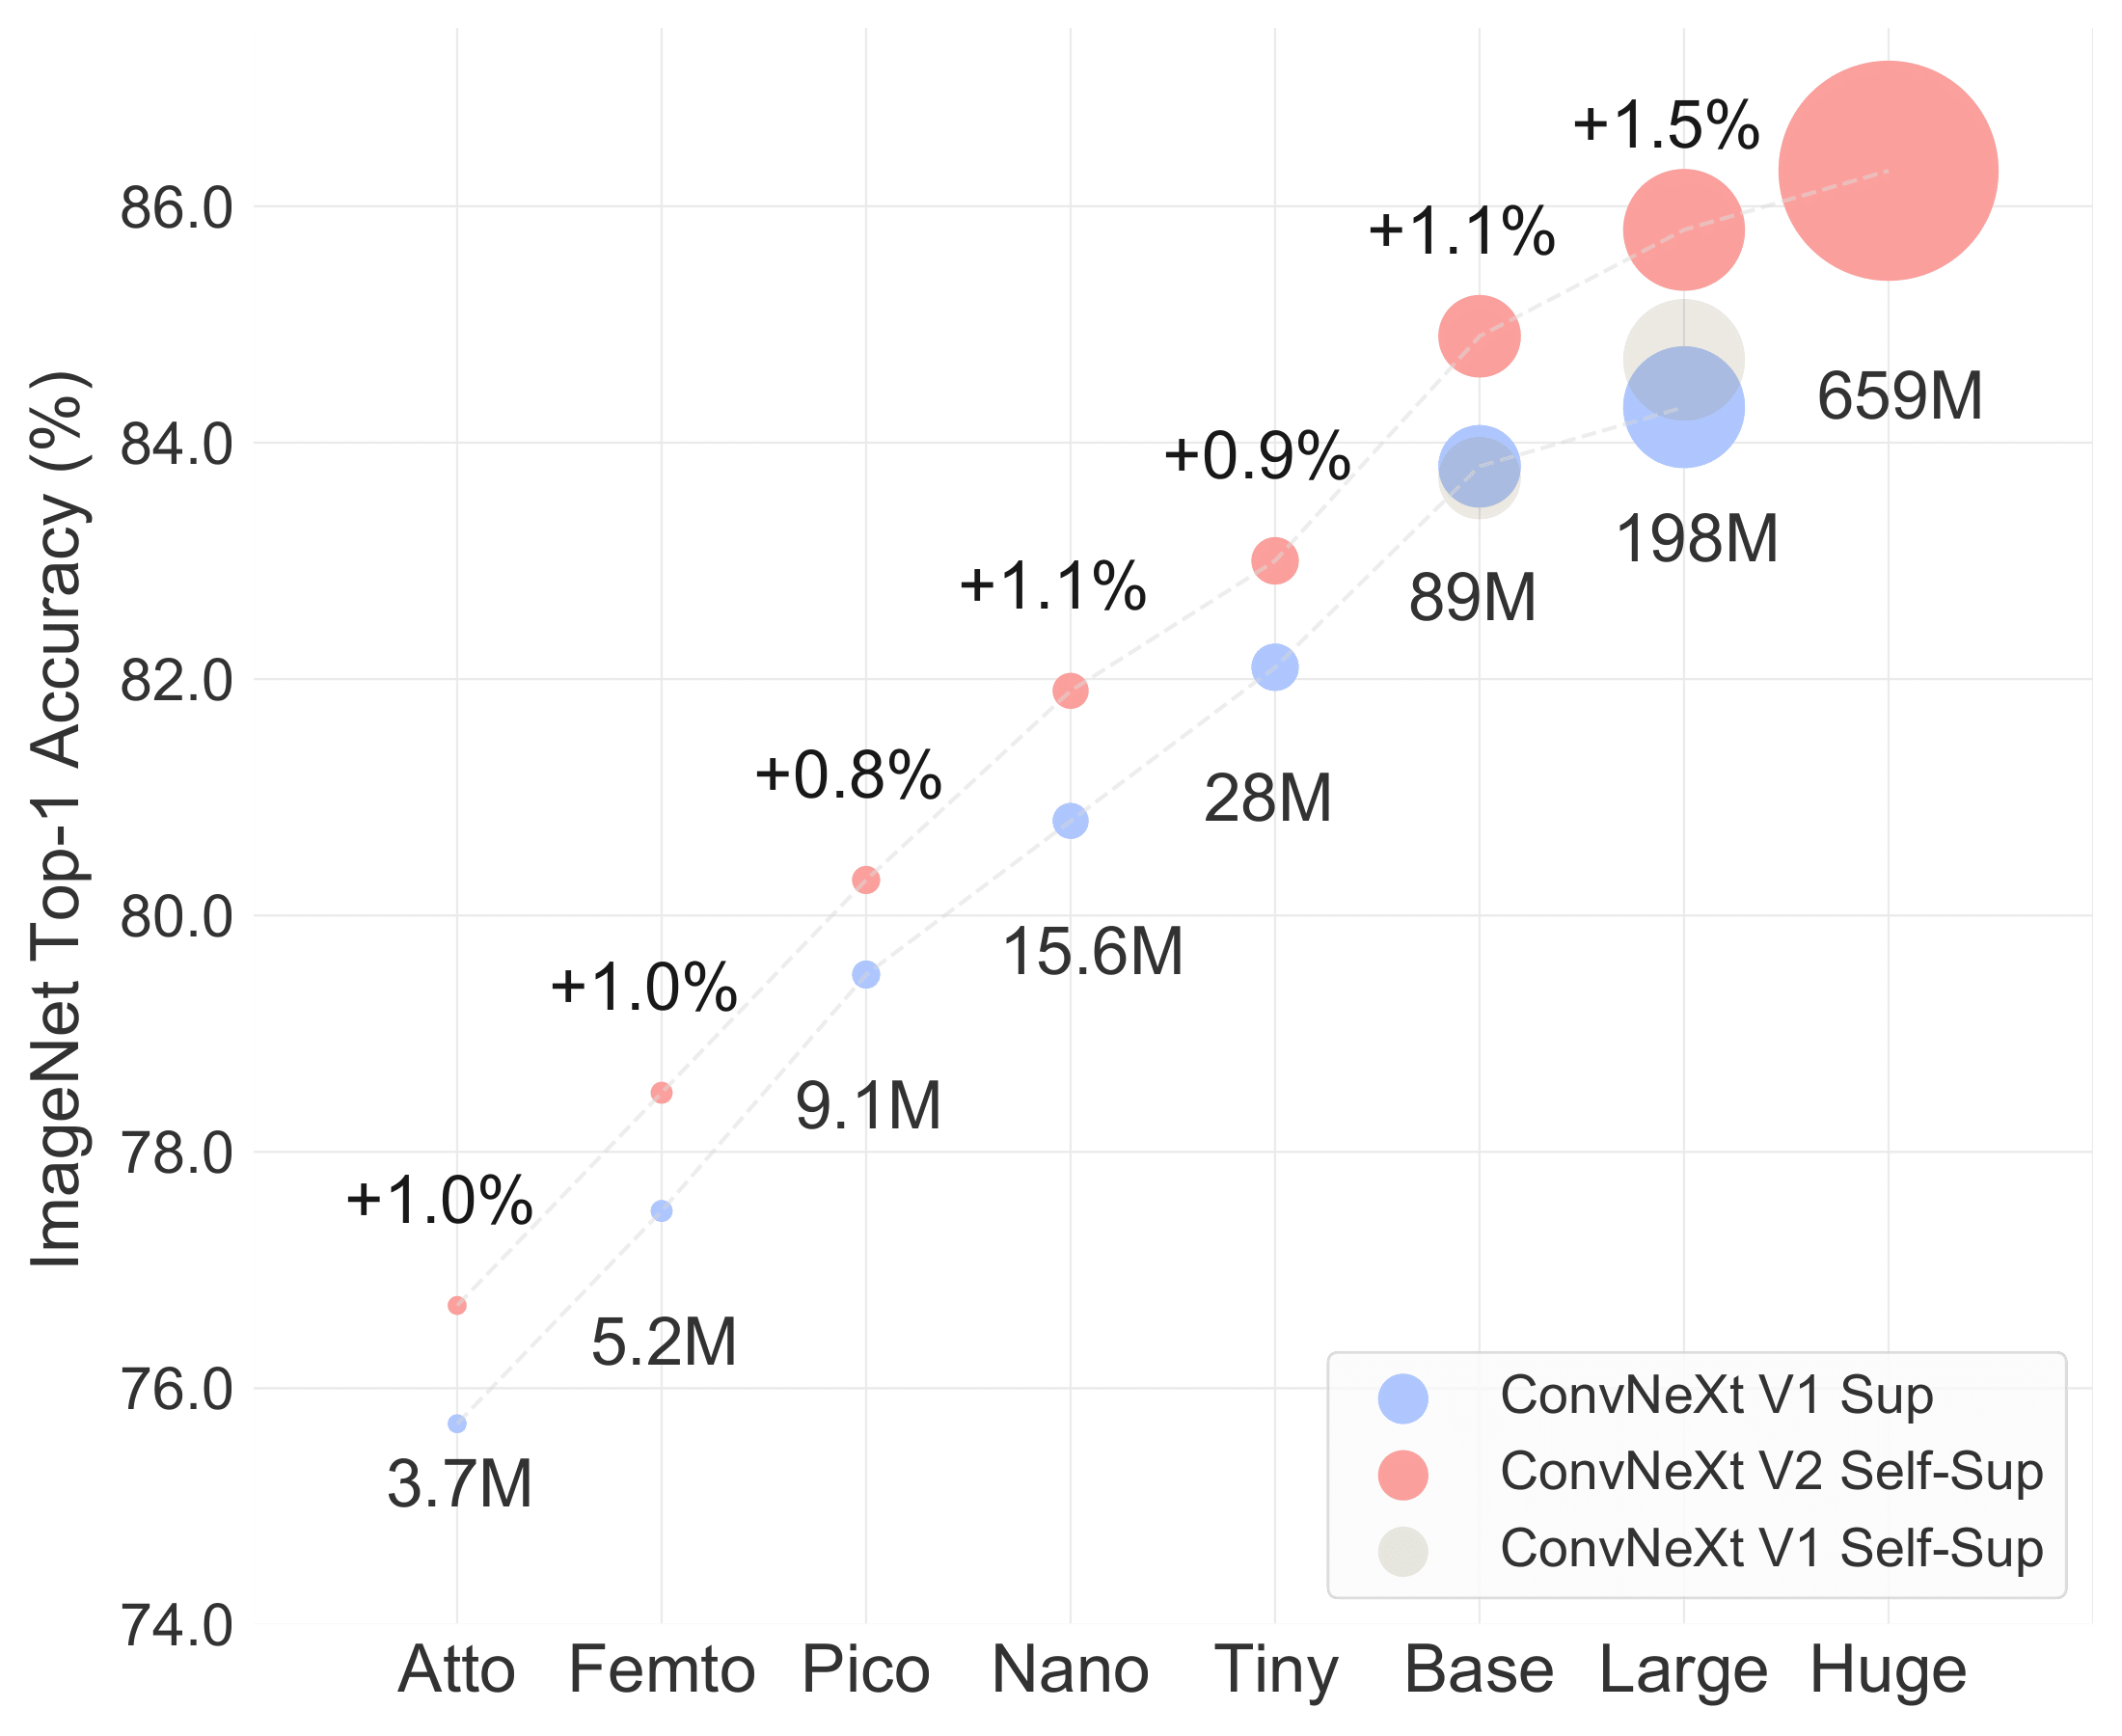
\includegraphics[width=0.82\textwidth]{figures/ml/scaling.png}
  \caption{Escalamiento de modelos ConvNeXtV2 y relación entre tamaño de red, capacidad representacional y desempeño. La figura muestra cómo la familia organiza variantes de distinta complejidad, desde configuraciones compactas hasta modelos de mayor escala. \textbf{Fuente:} Adaptado de Woo et al..}
  \label{fig:convnextv2-scaling}
\end{figure}

La Figura~\ref{fig:convnextv2-scaling} permite contextualizar la selección de una variante compacta dentro de la familia ConvNeXtV2 \citep{woo2023convnextv2}. En este trabajo se adopta \texttt{ConvNeXtV2\_atto}, la configuración más ligera de la familia, porque ofrece un compromiso adecuado entre capacidad representacional, estabilidad de exportación y costo de despliegue. Esta elección no busca maximizar el tamaño del extractor, sino preservar la integridad de la red durante la transformación desde PyTorch hacia ONNX y facilitar su distribución en entornos con recursos limitados. Aun con esta escala compacta, el backbone conserva profundidad suficiente para capturar textura, penumbra, fragmentación interna y extensión global del grupo solar \citep{woo2023convnextv2}. Esta característica es especialmente útil para la clasificación Zurich--McIntosh, donde las diferencias entre clases no dependen solo de la presencia de manchas, sino de patrones morfológicos sutiles como continuidad penumbral, compactación, separación longitudinal y distribución de manchas intermedias. Frente a CNN más antiguas, ConvNeXtV2 conserva el sesgo inductivo local de la convolución, favorable para texturas fotosféricas, pero incorpora mejoras de escalamiento y entrenamiento que lo acercan al rendimiento de arquitecturas modernas. Frente a transformadores visuales, mantiene una implementación más directa para recortes de tamaño moderado y se adapta de forma natural a salidas MLP multisalida para aprendizaje jerárquico.

\subsection{Modelos predictivos de la actividad solar}

El análisis de la actividad fotosférica ha evolucionado desde la simple observación morfológica hacia la construcción de marcos predictivos que buscan anticipar la evolución temporal del ciclo solar. Este problema es de naturaleza compleja, ya que el número, el área y la distribución latitudinal de las manchas solares responden a una modulación asimétrica y estocástica que dificulta los pronósticos de largo plazo \citep{pesnell2012predictions}. En la literatura actual, las estrategias para abordar esta variabilidad se dividen principalmente entre métodos de precursores físicos, modelos estadísticos de series temporales y, más recientemente, enfoques basados en aprendizaje automático, identificación dinámica y descomposición de señales \citep{clette2014revisiting}.

Dentro de los métodos operativos más consolidados, el uso de precursores basados en los campos polares y los índices geomagnéticos ha demostrado ser eficaz para estimar la amplitud del máximo de un ciclo con varios años de antelación \citep{schatten2005precursor,svalgaard2005polar}. Sin embargo, estos enfoques a menudo carecen de la resolución temporal necesaria para describir la evolución mensual de la actividad. Para subsanar esta limitación, se han desarrollado técnicas de filtrado adaptativo que permiten una actualización recursiva de las predicciones a medida que se disponen de nuevos registros mensuales.

El índice más utilizado para representar esa evolución temporal es el número de manchas solares o SSN, históricamente conocido como número de Wolf. En su formulación clásica, este índice combina el número de grupos solares observados y el número total de manchas individuales mediante una expresión del tipo $R=k(10g+s)$, donde $g$ representa los grupos, $s$ las manchas individuales y $k$ un factor de escala asociado al observador o instrumento. Su valor no debe interpretarse como un conteo físico directo, sino como un índice normalizado de actividad fotosférica que permite comparar observaciones realizadas bajo condiciones instrumentales y observacionales distintas \citep{clette2007wolf,clette2014revisiting}.

En este contexto, Podladchikova y Van der Linden \citep{podladchikova2012kalman} proponen una técnica de mejora basada en el filtro de Kalman adaptativo aplicada a predicciones del número de manchas solares suavizado. En una notación consistente con el modelo usado en la Sección~\ref{sec:forecast}, el pronóstico escalar puede formularse con un estado oculto $s_k\in\mathbb{R}$ asociado al SSN suavizado y una observación mensual $z_k\in\mathbb{R}$. La dinámica a priori se escribe como
\begin{equation}
\widehat{s}_{k}^{-}=\Phi_k\widehat{s}_{k-1},
\end{equation}
donde $\widehat{s}_{k}^{-}$ es la estimación previa al incorporar la observación del mes $k$ y $\Phi_k$ representa el cambio relativo esperado de la curva guía del ciclo. La incertidumbre asociada se propaga mediante
\begin{equation}
P_k^{-}=\Phi_k^{2}P_{k-1}+Q_k,
\end{equation}
donde $P_k^{-}$ es la varianza a priori y $Q_k$ representa el ruido de proceso.

Para construir la transición $\Phi_k$, el modelo retoma el perfil analítico de ciclo introducido por Hathaway, Wilson y Reichmann \citep{hathaway2010solarcycle}. Si $v$ denota el tiempo transcurrido desde el inicio efectivo del ciclo, la forma base puede escribirse como
\begin{equation}
f(v;a,b)=\frac{a v^{3}}{\exp\!\left(v^{2}/b^{2}\right)-0.71},
\end{equation}
donde $a$ controla la amplitud y $b$ regula la anchura temporal del ciclo. En consecuencia, la transición entre instantes consecutivos se define como
\begin{equation}
\Phi_k=\frac{f(v_k;a,b)}{f(v_{k-1};a,b)}.
\end{equation}
La actualización con la observación disponible se realiza mediante la ganancia de Kalman
\begin{equation}
K_k=P_k^{-}\left(P_k^{-}+R_k\right)^{-1},
\end{equation}
y la corrección del estado queda dada por
\begin{equation}
\widehat{s}_{k}=\widehat{s}_{k}^{-}+K_k\left(z_k-\widehat{s}_{k}^{-}\right),
\end{equation}
donde $R_k$ es la varianza del ruido de medición. Así, la salida escalar del bloque predictivo puede denotarse como $\mathrm{SSN}_{\mathrm{PVLK}}(t_k)=\widehat{s}_{k}$, manteniendo la misma convención empleada en la formulación metodológica.

Paralelamente al desarrollo de estos modelos estadísticos unidimensionales, el auge de la heliofísica computacional ha impulsado el uso de arquitecturas de redes neuronales y otros modelos de aprendizaje estadístico \citep{camporeale2019ml}. Estos trabajos sugieren que la predictibilidad del Sol puede mejorar sustancialmente si se consideran regularidades no lineales que los modelos empíricos tradicionales suelen omitir. No obstante, un desafío persistente en estos métodos es la integración de la información latitudinal de manera coherente con la física de la dinamo.

En este escenario, surge el interés por las técnicas de descomposición modal aplicadas a datos vectorizados. La Descomposición en Modos Dinámicos (DMD) resulta especialmente adecuada para reproducir fenómenos dinámicos a partir de múltiples observaciones, porque estima un operador que relaciona instantáneas consecutivas del sistema y permite reconstruir su evolución dominante. Esta propiedad explica su uso extendido en modelos físicos de mecánica de fluidos y sistemas complejos \citep{schmid2010dmd,kutz2016dmd}, así como su incorporación reciente en métodos de identificación dinámica para algoritmos iterativos y problemas numéricos de gran escala \citep{benitez2026adaptive}.

Desde esta perspectiva, la presente tesis adopta el DMD como una línea propia de modelado para explorar la evolución latitudinal de la actividad solar. La idea central no se desarrolla aquí como parte del estado del arte, sino que se retoma metodológicamente en la Sección~\ref{sec:forecast}: tratar el diagrama de Spörer como una secuencia de observaciones espacio-temporales y derivar, a partir de su reconstrucción dinámica, una tendencia global comparable con los pronósticos escalares tradicionales. De este modo, el DMD se introduce en esta revisión principalmente como antecedente conceptual y como motivación para la propuesta predictiva desarrollada posteriormente.